\documentclass[11pt]{article}

\usepackage{acl}

% Standard package includes
\usepackage{times}
\usepackage{latexsym}
\usepackage[T1]{fontenc}
\usepackage[utf8]{inputenc}
\usepackage{microtype}
% \usepackage{inconsolata}
\usepackage{graphicx}
\usepackage{booktabs}
\usepackage{amsmath}
\usepackage{amssymb}
\usepackage{enumitem}
\usepackage{subcaption}

% Tighten title box for two authors and prevent underfull page vertical stretching
\setlength\titlebox{4.8cm}
\raggedbottom

% Float placement parameters to prevent floats from drifting past sections
\renewcommand{\topfraction}{0.95}
\renewcommand{\bottomfraction}{0.95}
\renewcommand{\textfraction}{0.05}
\renewcommand{\floatpagefraction}{0.85}
\renewcommand{\dbltopfraction}{0.95}
\renewcommand{\dblfloatpagefraction}{0.85}

\title{ChartPRM: Process Reward Modeling and Step-Level Preference Optimization for Complex Multimodal Chart Reasoning}

\author{
  Yahor Lahunovich \\
  University of Heidelberg, \\
  Warsaw University of Technology \\\And
  Ertugrul Taparci \\
  University of Heidelberg \\
}

\begin{document}
\maketitle

% 1. Abstract
\begin{abstract}
Can a compact 3B vision-language model reason over complex scientific charts, not just read numbers off them? We study \texttt{Qwen2.5-VL-3B-Instruct} on two benchmarks: 500 reasoning problems from CharXiv and a matched pool from ChartQA. A multimodal LLM-as-a-judge (\texttt{muse-spark-1.1}) scores each reasoning step rather than only the final answer. Over 80\% of first errors happen within two steps, and once a step fails, the next fails 83\% of the time. Critique analysis of 2,920 failed steps points to perception, not arithmetic: axis and legend misreadings dominate. We train seven alignment methods on this signal (SFT, full DPO, Step-DPO, KTO, SimPO, Pareto-DPO, and SFT$\rightarrow$DPO) against the base model and ChartGemma. To keep this supervision from resting on one judge's scalar opinion, we cluster its critiques into a reward tree and select preference pairs by Pareto dominance across its criteria. That method wins on both benchmarks: Pareto-DPO reaches 30\% exact-match on CharXiv, ahead of a 26\% base, and 60\% on ChartQA after transfer, against a 43\% base, the largest gain of any method on either dataset. Chart reasoning in small models fails on perception rather than logic, and dominance-filtered process reward is what survives the move to a second dataset.
\end{abstract}

% 2. Introduction
\section{Introduction}
\label{sec:introduction}

Reasoning over scientific charts requires multimodal models to interleave visual perception (resolving dual axes, tick scales, and legend mappings) with symbolic deduction (computing rates and comparing extrema). Standard Outcome Reward Models (ORMs) provide sparse feedback only on the final answer \citep{ouyang2022instructgpt}, failing to isolate whether an error stems from an early visual misreading or downstream arithmetic. In contrast, Process Reward Models (PRMs) provide dense, step-by-step verification to enable granular credit assignment \citep{lightman2023prm}.

In this paper, we investigate a central hypothesis: \textit{Can a compact vision-language model reason effectively over complex scientific charts when aligned with only a small, process-supervised dataset?} Rather than relying on tens of thousands of annotations, we study whether fewer than 150 verified contrastive preference pairs suffice to align a compact model under consumer-grade compute constraints. A second question follows directly from the first: once such process supervision is built for one chart-QA benchmark, does it stay specific to that benchmark, or does it transfer, unmodified, to a second one?

We evaluate this hypothesis on the \textbf{CharXiv} benchmark \citep{wang2024charxiv}, and later test transfer on \textbf{ChartQA} \citep{masry2022chartqa}. Discarding surface-level descriptive queries, we isolate a stratified subset of \textbf{500 multi-step reasoning questions} from CharXiv spanning 8 academic domains and 62 chart types. Operating within a single 16GB Nvidia T4 GPU budget, we benchmark \texttt{Qwen2.5-VL-3B-Instruct} \citep{bai2025qwen25vl} using 4-bit NF4 quantization \citep{dettmers2023qlora} and LoRA \citep{hu2021lora}.

Using an LLM-as-a-judge (\texttt{muse-spark-1.1}) \citep{meta2026musespark, zheng2023judging} with rollout-level batching, we evaluate 1,274 rollouts (4,947 steps). Analyzing 2,920 refuted steps reveals two primary diagnostic findings:
\begin{enumerate}[noitemsep,topsep=0pt]
    \item \textbf{Perceptual Bottleneck}: Failures are overwhelmingly visual: axis/layout misreads (24.0\%) and series/color confusion (19.5\%) account for 43.5\% of failed steps, whereas pure arithmetic errors represent only 1.3\% (1 in 77 errors).
    \item \textbf{Catastrophic Cascades}: Errors emerge early: 79.7\% of failed traces break down in Steps 0--1. Once a step fails, the next step fails 82.7\% of the time ($P(S_{N+1}=0 \mid S_N=0) = 82.7\%$).
\end{enumerate}

Leveraging these diagnostics, we benchmark seven alignment strategies on a 100-question held-out set: SFT (70 traces), Full DPO (134 pairs) \citep{rafailov2023dpo}, Suffix Step-DPO (54 pairs) \citep{lai2024stepdpo}, KTO (84 pos / 252 neg) \citep{ethayarajh2024kto}, SFT$\rightarrow$DPO, the reference-free SimPO \citep{meng2024simpo}, and a Pareto-dominance-filtered variant of DPO introduced in this work. Confirming our small-data hypothesis, full-trajectory preference optimization is consistently the strongest paradigm: Full DPO reaches 29.0\% accuracy on just 134 pairs (+3.0 pp over the 26.0\% base), and Pareto-filtering the same pairs edges this further to 30.0\%, the best result on CharXiv. SFT enforces 100\% formatting compliance but lowers accuracy to 23.0\% via template rigidity, while KTO attains 66.0\% latent ground-truth recall in text but suffers structural format collapse.

A single binary judge score, however, is a coarse training signal: it cannot tell a rollout that misreads an axis apart from one that hallucinates a legend entry, even though both receive the same failing label. Motivated by Yin et al.'s Dynamic and Generalizable Process Reward Modeling (DG-PRM) \citep{yin2024dgprm}, we adapt this idea to chart reasoning: we distill the judge's failure critiques into a reward tree of 33 scored criteria grouped under the 9 error categories above, and instead of collapsing a rollout's scores to one scalar, we keep a 9-dimensional vector and accept a preference pair only when the correct rollout Pareto-dominates the incorrect one across every category at once. This is what produces the 30.0\% result. To test whether this dynamic judge is also generalizable, as DG-PRM's own name claims, we transfer the reward tree unmodified to ChartQA and retrain all seven methods there: the tree fires on ChartQA content at least as densely as on CharXiv, and Pareto-DPO wins by a wide margin, 60.0\% exact-match against a 43.3\% base, the largest gain of any method on either dataset. We additionally show the same judge is useful at inference time, without any training: reranking existing rollouts by step-level process reward reaches 27.5\% accuracy, ahead of majority-vote self-consistency (21.0\%) and random selection (18.4\%).

Our main contributions are:
\begin{itemize}[noitemsep,topsep=0pt]
    \item Validating the small-data alignment hypothesis on \texttt{Qwen2.5-VL-3B-Instruct} using 134 PRM preference pairs on a single T4 GPU.
    \item Establishing an empirical 9-class error taxonomy across 2,920 refuted steps, proving perceptual failures (43.5\%) dwarf arithmetic errors (1.3\%).
    \item Quantifying error cascade dynamics: $\sim$80\% of errors begin in Steps 0--1, propagating with an 82.7\% failure rate.
    \item Benchmarking seven alignment methods and mapping the Pareto frontier between structural compliance and latent reasoning recall.
    \item Adapting DG-PRM's reward tree and dynamic multi-criteria judge to chart reasoning, and using Pareto-dominance pair selection to obtain CharXiv's best result (30.0\%).
    \item Testing DG-PRM's generalizability claim directly: transferring the reward tree unmodified to ChartQA, where it fires as densely as on CharXiv and Pareto-DPO again wins decisively (60.0\% vs.\ 43.3\% base).
    \item Showing the same PRM judge is useful as a test-time verifier, reranking existing rollouts to beat majority-vote self-consistency and random selection.
\end{itemize}

% 4. The ChartPRM Framework (Core Implementation - 2 Pages)
\section{The ChartPRM Framework}
\label{sec:chartprm_framework}

The central goal of \textbf{ChartPRM} is to verify, diagnose, and align step-by-step visual reasoning on complex scientific charts. Scientific plots pack dense information into visual elements. Solving a reasoning question requires multiple distinct steps: locating the relevant panel, reading numerical axis scales, matching curve styles to legend labels, and performing logical comparisons.

ChartPRM decomposes this task into discrete reasoning steps, scores each step individually with a multimodal judge, and uses those step-level signals to guide preference optimization. Crucially, we also ask whether it is possible to align a compact 3B vision-language model using only a very small dataset of verified chart reasoning traces (fewer than 150 examples).

In this section, we describe the core components of the ChartPRM framework:
\begin{enumerate}[noitemsep,topsep=0pt]
    \item Structured step-by-step reasoning generation,
    \item Multimodal process reward modeling with rollout-level batching,
    \item Preference dataset curation and divergence slicing,
    \item Preference alignment objectives and training setup,
    \item DynamicPRM adaptive process reward modeling, and
    \item Test-time verification and candidate search.
\end{enumerate}

\subsection{Structured Step-by-Step Reasoning Protocol}
\label{subsec:reasoning_protocol}
To enable step-level verification, the vision-language model must generate reasoning traces that can be parsed into discrete steps. We use a structured Chain-of-Thought prompt \citep{wei2022cot} that instructs the model to break down its reasoning into sequential steps and end with a clear final answer:
\begin{quote}
\small
\texttt{Solve the chart reasoning question step by step. Structure your answer strictly as follows:\\
Step 1: <visual observation>\\
Step 2: <intermediate reading or deduction>\\
...\\
Final Answer: <concise answer>}
\end{quote}

We enforce three practical formatting rules:
\begin{itemize}[noitemsep,topsep=0pt]
    \item Each step must start with a explicit label (\texttt{Step 1:}, \texttt{Step 2:}, etc.).
    \item The final prediction must appear on its own line after \texttt{Final Answer:}, without markdown asterisks.
    \item The model must not include conversational filler (such as ``Certainly! Here is my analysis'').
\end{itemize}

To create a diverse pool of candidate solutions, we sample rollouts using temperature $\tau = 0.7$ and top-$p = 0.9$. For each question in the training pool, we sample up to four candidate rollouts. Across the 500 CharXiv \citep{wang2024charxiv} reasoning questions, this procedure generates 1,274 complete rollout trajectories.

We evaluate each rollout with an automated parser that extracts the prediction following \texttt{Final Answer:} and applies lowercase whitespace normalization to measure exact match against the ground truth.

\subsection{Multimodal Process Reward Modeling}
\label{subsec:prm_judge}
Once rollouts are generated, we evaluate each intermediate reasoning step using a multimodal LLM-as-a-judge \citep{zheng2023judging}. We employ \texttt{muse-spark-1.1} \citep{meta2026musespark} as our judge model. 

Evaluating each step in an individual API call would require repeatedly uploading the high-resolution chart image for every step, quickly exhausting API token allowances. To address this constraint, we implement \textit{rollout-level batching}: we downscale the chart image to a maximum dimension of 512 pixels (preserving visual legibility while reducing token costs) and evaluate all reasoning steps of a rollout within a single multimodal API request.

The judge receives:
\begin{enumerate}[noitemsep,topsep=0pt]
    \item The chart image $I$ (resized to $\le 512$\,px),
    \item The question text $q$,
    \item The reference ground-truth answer $y^*$, and
    \item The full sequence of generated steps $(y_1, \dots, y_T)$.
\end{enumerate}

The judge evaluates each step sequentially in context and returns a structured JSON array containing two fields per step:
\begin{itemize}[noitemsep,topsep=0pt]
    \item \textbf{Binary Step Score ($s_t \in \{0, 1\}$):} The judge assigns $s_t = 1$ if the visual grounding and deduction in Step $t$ are factually correct. It assigns $s_t = 0$ if the step contains an axis misreading, color confusion, hallucinated label, or arithmetic mistake.
    \item \textbf{Natural Language Critique:} For each failed step ($s_t = 0$), the judge provides a concise critique explaining the specific visual or logical failure (for example: ``The model misreads the logarithmic y-axis scale as linear, estimating 40 instead of 10'').
\end{itemize}

We define the overall process reward of a complete reasoning trajectory $\tau$ as the mean score across all its steps:
\begin{equation}
    R(\tau) = \frac{1}{T} \sum_{t=1}^T s_t
    \label{eq:process_reward}
\end{equation}
A trajectory is considered \textit{fully verified} only if every step receives a passing score ($R(\tau) = 1.0$). If any step fails, the trajectory receives $R(\tau) < 1.0$.

\subsection{Preference Dataset Curation and Step Slicing}
\label{subsec:dataset_curation}
From the 1,274 judged rollouts (comprising 4,947 individual steps), we curate training datasets for five distinct alignment methods:

\textbf{1. Supervised Fine-Tuning (SFT) Dataset:} We select only rollouts that achieve a perfect process score ($R(\tau) = 1.0$) and also produce the correct final answer. This strict filter yields 70 gold-standard reasoning rollouts. Because every step is verified by the judge, the model is trained exclusively on factually grounded visual reasoning.

\textbf{2. Sequence DPO Preference Pairs:} For each question where multiple rollouts were sampled, we construct pairwise comparisons $(y_w, y_l)$. The chosen rollout $y_w$ has a higher process reward ($R(y_w) > R(y_l)$) or reaches the correct final answer when $y_l$ does not. This yields 134 chosen-rejected sequence pairs across the training pool.

\textbf{3. Step-DPO Suffix Slicing:} In standard sequence DPO, the entire rejected response is penalized equally. However, our trajectory analysis reveals that rejected rollouts often start with completely correct steps. Penalizing early correct steps teaches the model the wrong lesson. 

To solve this credit assignment problem, Step-DPO isolates the first point of divergence. For each pair $(y_w, y_l)$, we compare steps sequentially to identify the first step index $t^*$ where the two traces diverge or where $y_l$ makes its first mistake:
\begin{equation}
    t^* = \min \{ t \mid y_{w,t} \neq y_{l,t} \text{ or } s_t(y_l) = 0 \}
\end{equation}
We keep the shared prefix $y_{<t^*}$ as prompt context, but compute the preference loss strictly over the divergent suffix starting at $t^*$. This yields 54 clean, prefix-aligned step pairs.

\textbf{4. KTO Unpaired Dataset:} Unlike DPO, Kahneman-Tversky Optimization does not require paired rollouts for the exact same prompt. We split rollouts into desirable and undesirable pools based on their process score and answer accuracy. We collect 84 desirable rollouts ($R \ge 0.75$ and correct final answer) and 252 undesirable rollouts ($R < 0.5$ or wrong answer), establishing a 1:3 positive-to-negative ratio.

\subsection{Preference Alignment Objectives and Training Setup}
\label{subsec:alignment_objectives}

\begin{table}[t]
\centering
\footnotesize
\setlength{\tabcolsep}{2.5pt}
\begin{tabular}{lcccc}
\toprule
\textbf{Method} & \textbf{Data Size} & \textbf{Epochs} & \textbf{LR} & \textbf{Time} \\
\midrule
SFT & 70 traces & 1 & $1\times 10^{-5}$ & 12 min \\
Full DPO & 134 pairs & 1 & $1\times 10^{-5}$ & 22 min \\
Step-DPO & 54 pairs & 2 & $1\times 10^{-5}$ & 15 min \\
KTO & 84 pos / 252 neg & 2 & $2\times 10^{-6}$ & 35 min \\
SFT$\rightarrow$DPO & 134 pairs & 1 & $2\times 10^{-6}$ & 24 min \\
SimPO & 134 pairs & 1 & $1\times 10^{-6}$ & -- \\
Pareto-DPO & 154 pairs & 1 & $1\times 10^{-5}$ & -- \\
\bottomrule
\end{tabular}
\caption{\textbf{Fine-Tuning Configurations under 16GB GPU Budget.} All models are trained with 4-bit LoRA adaptation ($r=16$) on \texttt{Qwen2.5-VL-3B-Instruct} \citep{bai2025qwen25vl}. SimPO and Pareto-DPO are described in this subsection and \S\ref{subsec:dynamic_prm} respectively.}
\label{tab:training_setup}
\end{table}

Using the curated datasets, we align the policy model $\pi_\theta$ against a frozen reference policy $\pi_{\text{ref}}$ (the base unaligned instruct model). All models are fine-tuned under a strict 16GB VRAM budget on an Nvidia Tesla T4 or Tesla P100 GPU on Kaggle, using 4-bit NF4 quantization \citep{dettmers2023qlora} and LoRA adapters \citep{hu2021lora} with rank $r=16$ on \texttt{Qwen2.5-VL-3B-Instruct} \citep{bai2025qwen25vl}. Table~\ref{tab:training_setup} summarizes the training configurations, dataset sizes, learning rates, and wall-clock runtimes. Peak GPU memory remains under 14.2\,GB throughout training.

We investigate seven alignment paradigms. The first five use the datasets curated in \S\ref{subsec:dataset_curation}; the remaining two, SimPO and Pareto-DPO, are introduced here and in \S\ref{subsec:dynamic_prm}.

\textbf{1. Supervised Fine-Tuning (SFT):} Following standard alignment pipelines \citep{ouyang2022instructgpt}, supervised fine-tuning serves as our initial demonstration baseline, maximizing the log-likelihood of verified gold reasoning steps (Equation~\ref{eq:sft_loss}, \ref{sec:appendix_objectives}). This teaches the model the desired formatting structure, but provides no negative feedback on what errors to avoid.

\textbf{2. Full-Sequence DPO:} Sequence-level Direct Preference Optimization \citep{rafailov2023dpo} optimizes a Bradley-Terry preference model directly over token probabilities:
\begin{align}
    \mathcal{L}_{\text{DPO}}(\theta; \pi_{\text{ref}}) = -\mathbb{E} \Big[ \log \sigma \Big( & \beta \log \frac{\pi_\theta(y_w \mid x)}{\pi_{\text{ref}}(y_w \mid x)} \nonumber \\
    {} - & \beta \log \frac{\pi_\theta(y_l \mid x)}{\pi_{\text{ref}}(y_l \mid x)} \Big) \Big]
    \label{eq:dpo_loss}
\end{align}
where $\sigma$ is the sigmoid function, and $\beta = 0.1$ controls the strength of the KL regularization penalty.

\textbf{3. Suffix Step-DPO:} Suffix Step-DPO \citep{lai2024stepdpo} applies the DPO loss only to the divergent suffix, masking tokens in the shared prefix $y_{<t^*}$ out of the gradient (Equation~\ref{eq:stepdpo_loss}, \ref{sec:appendix_objectives}). The loss focuses entirely on correcting the initial visual mistake.

\textbf{4. Kahneman-Tversky Optimization (KTO):} KTO \citep{ethayarajh2024kto} aligns models using unpaired data via a prospect-theoretic utility function over the implicit reward $\hat{r}_\theta(x, y) = \log \frac{\pi_\theta(y \mid x)}{\pi_{\text{ref}}(y \mid x)}$ (Equation~\ref{eq:kto_loss}, \ref{sec:appendix_objectives}).

\textbf{5. Two-Stage SFT$\rightarrow$DPO:} We also evaluate a sequential pipeline where the model is first fine-tuned on verified gold traces with SFT for one epoch, and then aligned with sequence DPO using the SFT checkpoint as both the starting policy and the reference policy $\pi_{\text{ref}}$.

\textbf{6. SimPO:} Simple Preference Optimization \citep{meng2024simpo} removes the reference model entirely, replacing the KL term with the policy's own length-normalized log-probability and a target margin $\gamma$ (Equation~\ref{eq:simpo_loss}, \ref{sec:appendix_objectives}). Because no reference forward pass is needed, SimPO trains on half the forward passes per step that DPO requires. We use the same 134 full-trajectory pairs as Full DPO, $\beta = 2.0$, and $\gamma/\beta = 0.5$, isolating training objective as the only variable against Full DPO.

\textbf{7. Pareto-DPO:} Trained with the identical loss and hyperparameters as Full DPO (Equation~\ref{eq:dpo_loss} in this subsection), but on a differently constructed pair set: instead of the single-scalar chosen/rejected split from \S\ref{subsec:dataset_curation}, pairs are kept only when the correct rollout Pareto-dominates the incorrect one across a 9-dimensional vector of category-level scores. \S\ref{subsec:dynamic_prm} describes how this vector and the resulting 154 pairs are constructed.

\subsection{DynamicPRM}
\label{subsec:dynamic_prm}

A single binary score per step, as used in \S\ref{subsec:prm_judge}, cannot distinguish an axis misreading from a hallucinated legend entry: both simply receive $s_t = 0$. Motivated by Yin et al.'s Dynamic and Generalizable Process Reward Modeling (DG-PRM) \citep{yin2024dgprm}, we replace this single scalar with a structured, multi-criteria reward built from the judge's own failure language rather than imposed a priori.

\textbf{Reward Tree Construction:} We reuse the 9 error categories from the taxonomy in \S\ref{subsec:perceptual_bottleneck} as parent nodes (\textit{other/unspecified} excluded, as a catch-all rather than a criterion). Within each parent, we cluster the corresponding failure critiques by their MiniLM sentence embeddings ($k$-means, $k$ scaled to category size), merge near-duplicate sub-clusters (cosine distance $\le 0.14$), and distill each surviving child into a general rubric statement via one LLM call per parent. This yields \textbf{33 scored criteria} under 9 parents, built entirely from data already collected in \S\ref{subsec:perceptual_bottleneck}, requiring only 9 new API calls for distillation.

\textbf{Dynamic Multi-Criteria Judge:} For each step, the judge is shown the full 33-criterion tree once and self-selects which criteria apply, scoring each on a 1--3 scale, blind to the ground-truth answer (unlike the judge in \S\ref{subsec:prm_judge}). At full scale (309 training-pool questions, 1,199 rollouts, 4,652 steps), the judge selects 3.85 criteria per step on average and never returns an empty selection, indicating the tree is neither too narrow nor irrelevant to the failures it was built from. Collapsing these scores to one mean does not significantly outperform the original binary judge as a training signal (-2.6 pp, not significant). The dynamic judge earns its keep elsewhere, in exposing a 9-dimensional failure profile per rollout that a single scalar cannot represent.

\textbf{Pareto-Dominance Pair Selection:} Rather than reducing a rollout's scores to a mean, we retain the 9-dimensional vector, one score per parent category. A preference pair $(y_w, y_l)$ is kept only when $y_w$ Pareto-dominates $y_l$: at least as good on every category and strictly better on one. This discards pairs where the two rollouts trade off across different failure axes (one hallucinates less but misreads the axis more, say), a case a single scalar cannot distinguish from a clean win. Applied to the full 309-question pool, this yields \textbf{154 pairs}, trained with the identical DPO trainer and hyperparameters as Full DPO (Equation~\ref{eq:dpo_loss}). The result is CharXiv's best system at \textbf{30.0\% exact-match} (Table~\ref{tab:main_benchmark}), narrowly ahead of Full DPO's 29.0\%, though the difference is not statistically significant.

\textbf{Generalization to ChartQA:} DG-PRM's name claims the resulting reward is not just dynamic but \textit{generalizable}. We test this directly rather than assume it: the 33-criterion tree, built entirely from CharXiv judge critiques, is applied unmodified to 612 rollouts generated on a disjoint pool of ChartQA \citep{masry2022chartqa} questions, with no retuning and no new tree construction. Every step returns at least one applicable criterion (0\% empty selections, matching CharXiv), all 33 criteria fire at least once, and the average selection density is if anything higher than on CharXiv (4.21 vs.\ 3.85 criteria per step). Rebuilding preference pairs and retraining Pareto-DPO on ChartQA reproduces the CharXiv result decisively: \textbf{60.0\% exact-match} against a 43.3\% base, the largest margin of any of the seven methods on either dataset (\S\ref{subsec:alignment_benchmark}). Because the tree transfers without modification, this improvement cannot be attributed to retuning on ChartQA itself, and is, to our knowledge, the first evidence that a DG-PRM-style reward survives a change of dataset rather than only a change of model.

\subsection{Test-Time Verification and Search}
\label{subsec:test_time_verification}

Every use of the PRM judge so far is offline: it only shapes which traces enter a training set. A classical PRM use case is different, reranking a fixed pool of already-generated candidates at inference time \citep{lightman2023prm}, with no additional training. We test whether the judge is useful there too, using rollouts that already exist from \S\ref{subsec:reasoning_protocol}, no new generation.

For each of 309 training-pool questions with at least two rollouts, we compare three ways to pick a final answer from the candidate pool: uniform random selection, majority-vote self-consistency \citep{wang2023selfconsistency}, and PRM best-of-$N$, which picks the rollout with the highest mean step-level process reward $R(\tau)$ (Equation~\ref{eq:process_reward}). Table~\ref{tab:best_of_n} reports holdout exact-match for each strategy (visualized in Figure~\ref{fig:prm_best_of_n}, Appendix~\ref{sec:appendix_diagnostics}), alongside an oracle upper bound (a correct rollout exists somewhere in the pool for that question).

PRM best-of-$N$ reaches \textbf{27.5\%}, ahead of majority-vote self-consistency (21.0\%, +6.5 pp) and random selection (18.4\%, +9.1 pp). The oracle bound of 44.0\% shows substantial headroom remains: a correct rollout is available for 100\% of questions by construction, but the judge only identifies it 62.5\% of the time when one exists (27.5 / 44.0). Majority vote, by contrast, cannot exploit this headroom at all when the correct answer is a minority position among sampled rollouts, which is common at $\tau = 0.7$ sampling temperature. This establishes the judge as useful beyond its role as a training-data labeler: the same step-level signal that curates preference pairs in \S\ref{subsec:dynamic_prm} also improves accuracy directly at inference time, without any additional fine-tuning.

\begin{table}[t]
\centering
\footnotesize
\setlength{\tabcolsep}{2.6pt}
\begin{tabular}{lccc}
\toprule
\textbf{Strategy} & \textbf{Holdout EM} & \textbf{$\Delta$ vs.\ Rand} & \textbf{Solvable} \\
\midrule
Uniform Random & 18.4\% & -- & 41.8\% \\
Majority Vote & 21.0\% & +2.6 pp & 47.7\% \\
\textbf{PRM Best-of-$N$} & \textbf{27.5\%} & \textbf{+9.1 pp} & \textbf{62.5\%} \\
\midrule
\textit{Oracle Bound} & \textit{44.0\%} & \textit{+25.6 pp} & \textit{100.0\%} \\
\bottomrule
\end{tabular}
\caption{\textbf{Test-Time Verifier Performance ($N=309$ multi-candidate questions).} Selecting candidates by step-level process reward outperforms self-consistency by +6.5 pp.}
\label{tab:best_of_n}
\end{table}

% 4. Results and Analysis
\section{Results and Analysis}
\label{sec:results_analysis}

We evaluate the empirical performance of multimodal chart reasoning across four dimensions: reasoning trajectory dynamics, failure mode taxonomy, preference alignment effectiveness, and cross-dataset generalization. First, we examine multi-step rollouts from the unaligned base model, tracking the accuracy cliff and error cascades across reasoning depth (\S\ref{subsec:trajectory_dynamics}). Second, we analyze 2,920 refuted reasoning steps to establish an empirical error taxonomy (\S\ref{subsec:perceptual_bottleneck}), demonstrating that failures stem overwhelmingly from visual perception rather than arithmetic. Third, we benchmark seven preference-aligned policy models on held-out scientific reasoning problems (\S\ref{subsec:alignment_benchmark}) and analyze the Pareto trade-off between reasoning accuracy and output structure compliance (\S\ref{subsec:accuracy_structure_tradeoff}). Fourth, we retrain and re-evaluate all seven methods on a second, disjoint benchmark, ChartQA, to test whether any of these findings are specific to CharXiv (\S\ref{subsec:chartqa_generalization}).

\subsection{Reasoning Trajectory Dynamics and Error Cascades}
\label{subsec:trajectory_dynamics}

\begin{figure*}[t]
  \centering
  \begin{subfigure}{0.49\textwidth}
    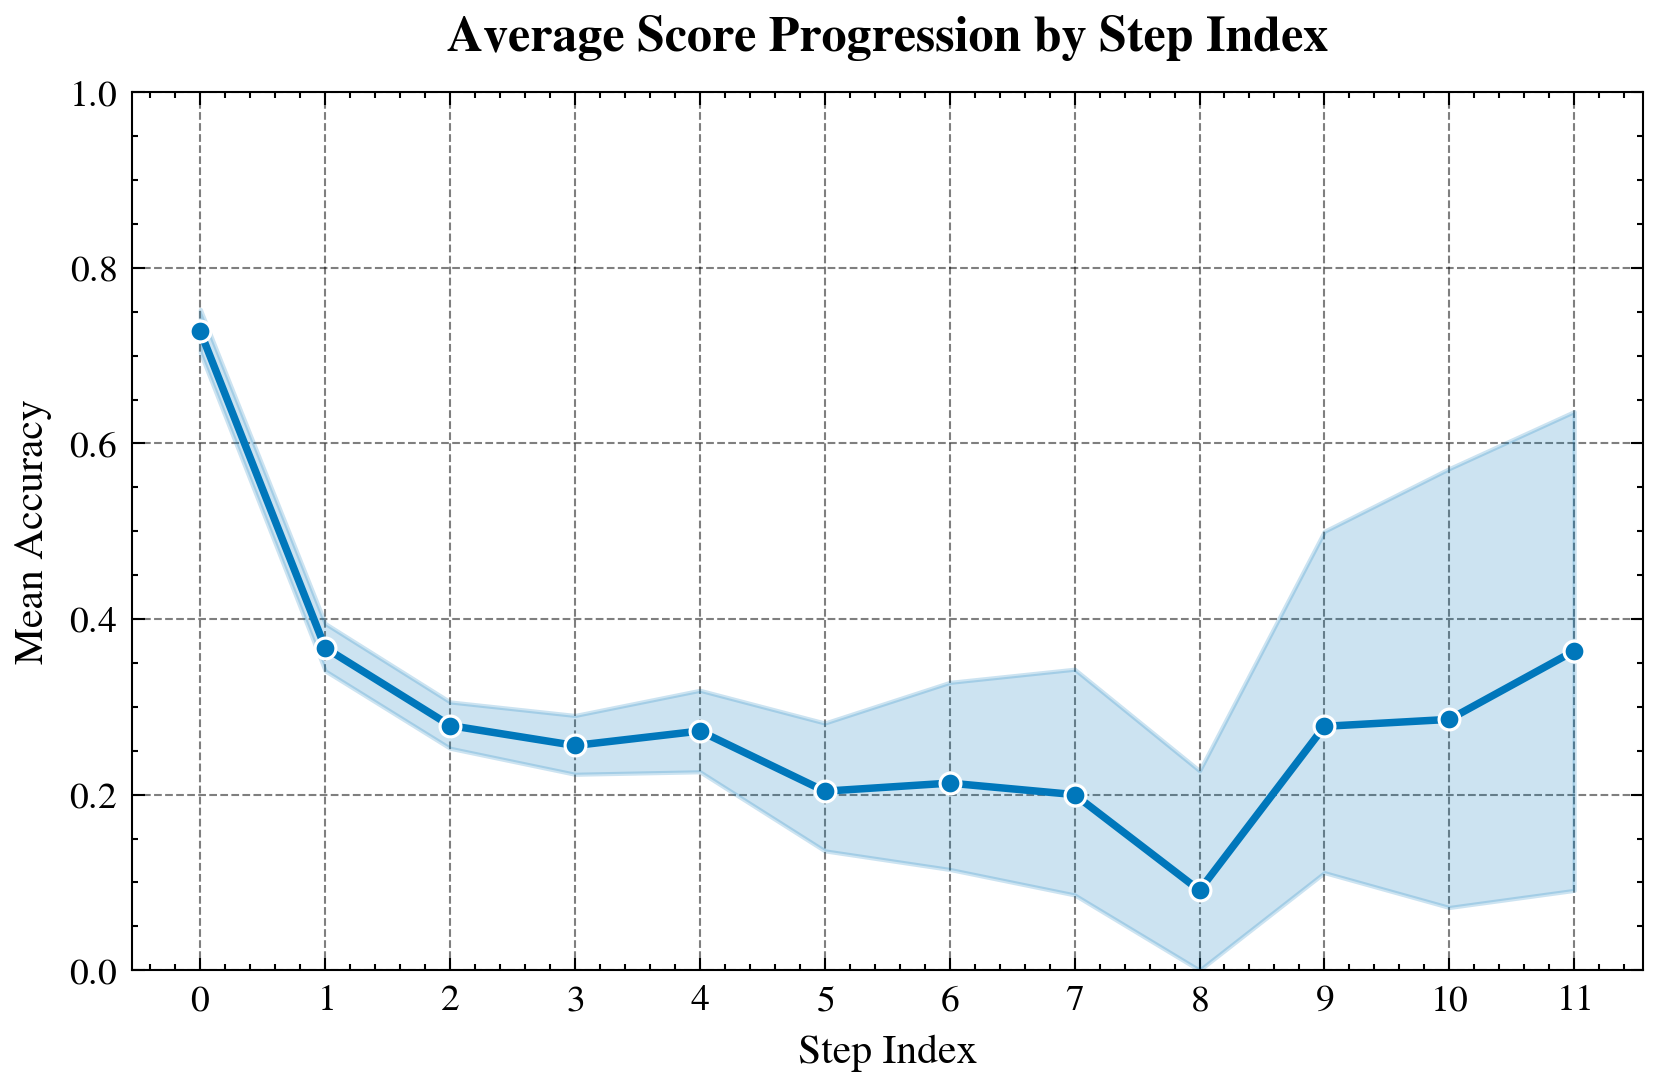
\includegraphics[width=\textwidth]{../charts/report_selected/02_score_progression.png}
    \caption{Step Score Cliff by Reasoning Depth}
    \label{fig:score_cliff}
  \end{subfigure}\hfill
  \begin{subfigure}{0.49\textwidth}
    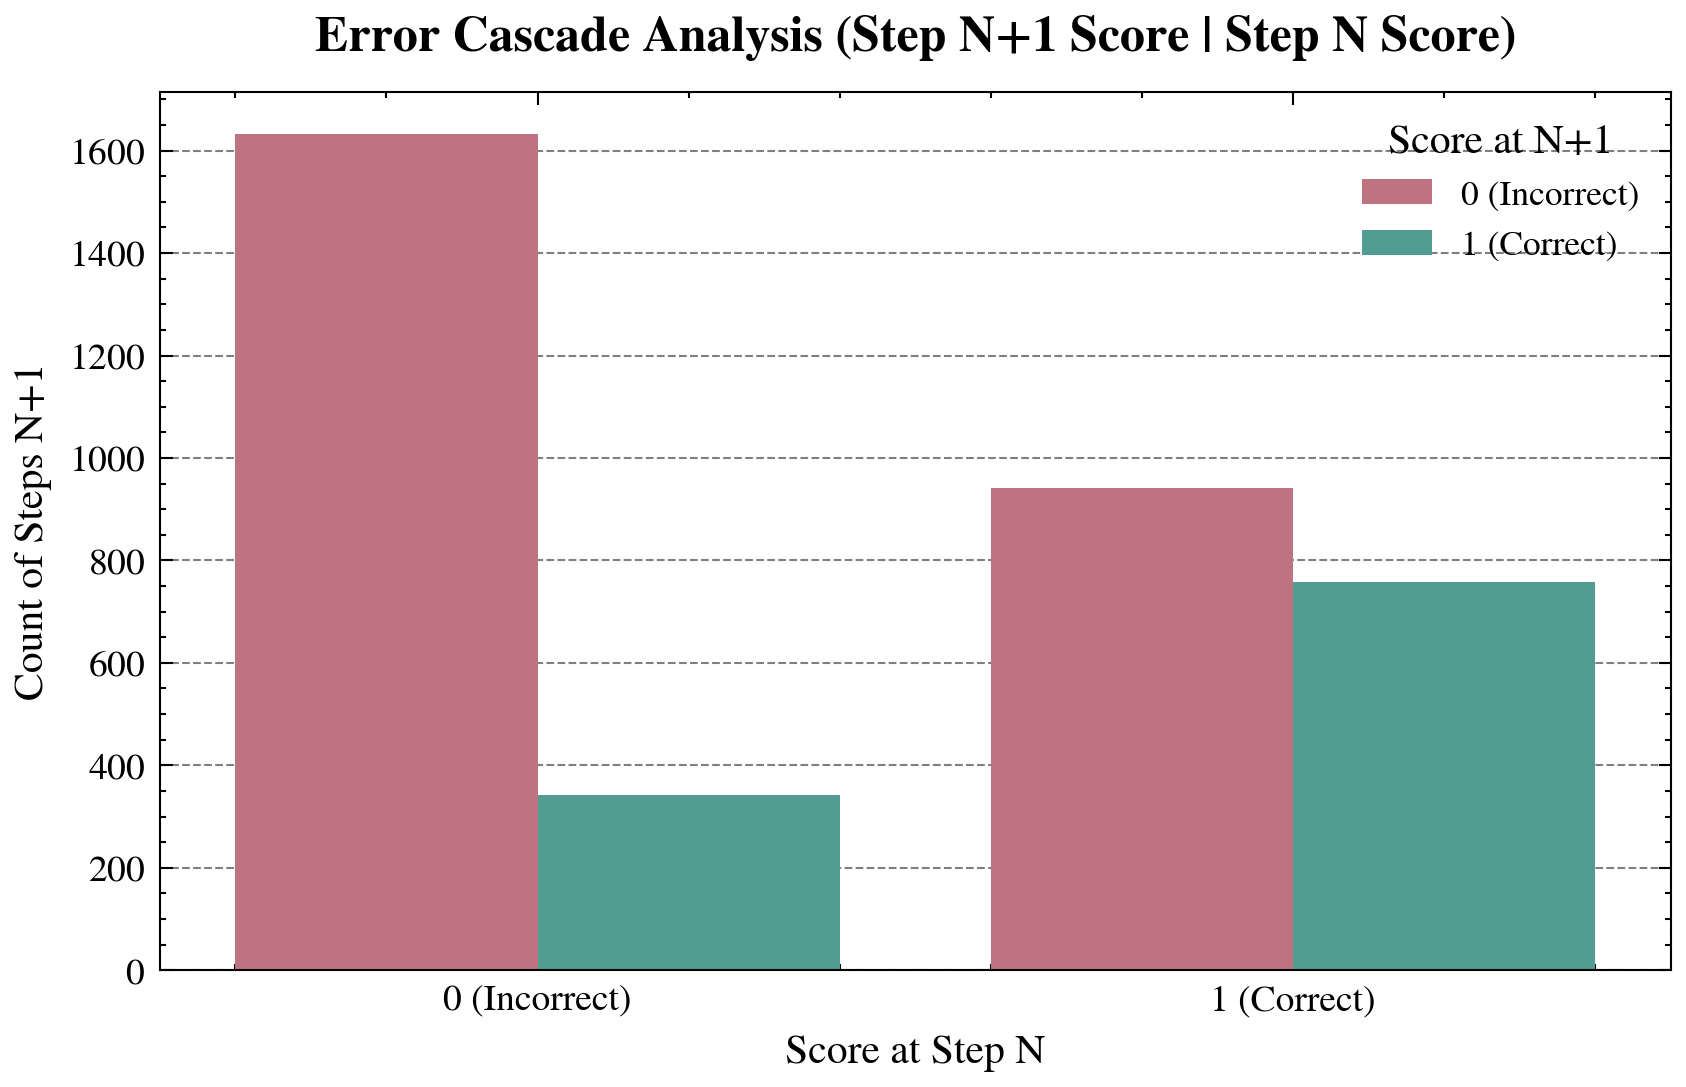
\includegraphics[width=\textwidth]{../charts/report_selected/08_error_cascade.png}
    \caption{Error Cascade Transition Probabilities}
    \label{fig:error_cascade}
  \end{subfigure}
  \caption{\textbf{Reasoning Trajectory Dynamics.} (a) Step accuracy plummets from 73\% at Step 0 to 26\% at Step 3. (b) When a step fails, the next step also fails 82.7\% of the time, proving that early visual mistakes cascade catastrophically.}
  \label{fig:trajectory_dynamics}
\end{figure*}

We analyze 1,274 reasoning rollouts generated by \texttt{Qwen2.5-VL-3B-Instruct} \citep{bai2025qwen25vl} across the 500 CharXiv \citep{wang2024charxiv} reasoning problems. Our multimodal judge evaluated all 4,947 individual reasoning steps. Figure~\ref{fig:trajectory_dynamics} illustrates the score progression and step transition dynamics (with complete trajectory statistics tabulated in Table~\ref{tab:trajectory_stats}, Appendix~\ref{sec:appendix_diagnostics}).

\textbf{The Reasoning Cliff:} As shown in Figure~\ref{fig:trajectory_dynamics}(a), reasoning quality drops sharply as the reasoning chain gets longer. At Step 0 (the initial setup or visual inspection), the model achieves a 73.0\% pass rate. However, accuracy falls to 43.1\% at Step 1 and plummets to 26.3\% by Step 3. Overall, only 12.1\% of all rollouts (154 out of 1,274) complete all steps without a single mistake. Multi-step chart reasoning requires sequential deductions: identifying relevant panels, reading axis values, matching curves to legends, and comparing numerical trends. For a compact 3B model, maintaining visual grounding becomes increasingly difficult at each subsequent step.

\textbf{The 82.7\% Error Cascade:} What happens when a step fails? Figure~\ref{fig:trajectory_dynamics}(b) (and Table~\ref{tab:trajectory_stats}) reveals an important failure dynamic: when a step fails ($s_t = 0$), the immediate next step also fails \textbf{82.7\% of the time} ($P(S_{N+1}=0 \mid S_N=0) = 82.7\%$). The model recovers to a valid step in only 17.3\% of cases. Furthermore, \textbf{79.7\%} of all flawed rollouts make their first mistake in the very first two steps (31.0\% at Step 0, and 48.8\% at Step 1).

\textbf{Why Process Verification Matters:} These observations explain how vision-language models fail on charts. Errors do not accumulate slowly near the end of the response. Instead, the model stumbles right at the beginning. An initial misread acts as a poisoned premise: all downstream steps perform calculations on false coordinates or misidentified curves. This dynamic strongly justifies process reward modeling \citep{lightman2023prm}. An outcome reward model (ORM) only notices that the final answer is wrong. In contrast, a process reward model (PRM) pinpoints the exact step where grounding failed, allowing verifiers to stop cascading errors before they spread.

\subsection{The Perceptual Bottleneck: Why Chart Reasoning Fails}
\label{subsec:perceptual_bottleneck}

\begin{figure}[t]
  \centering
  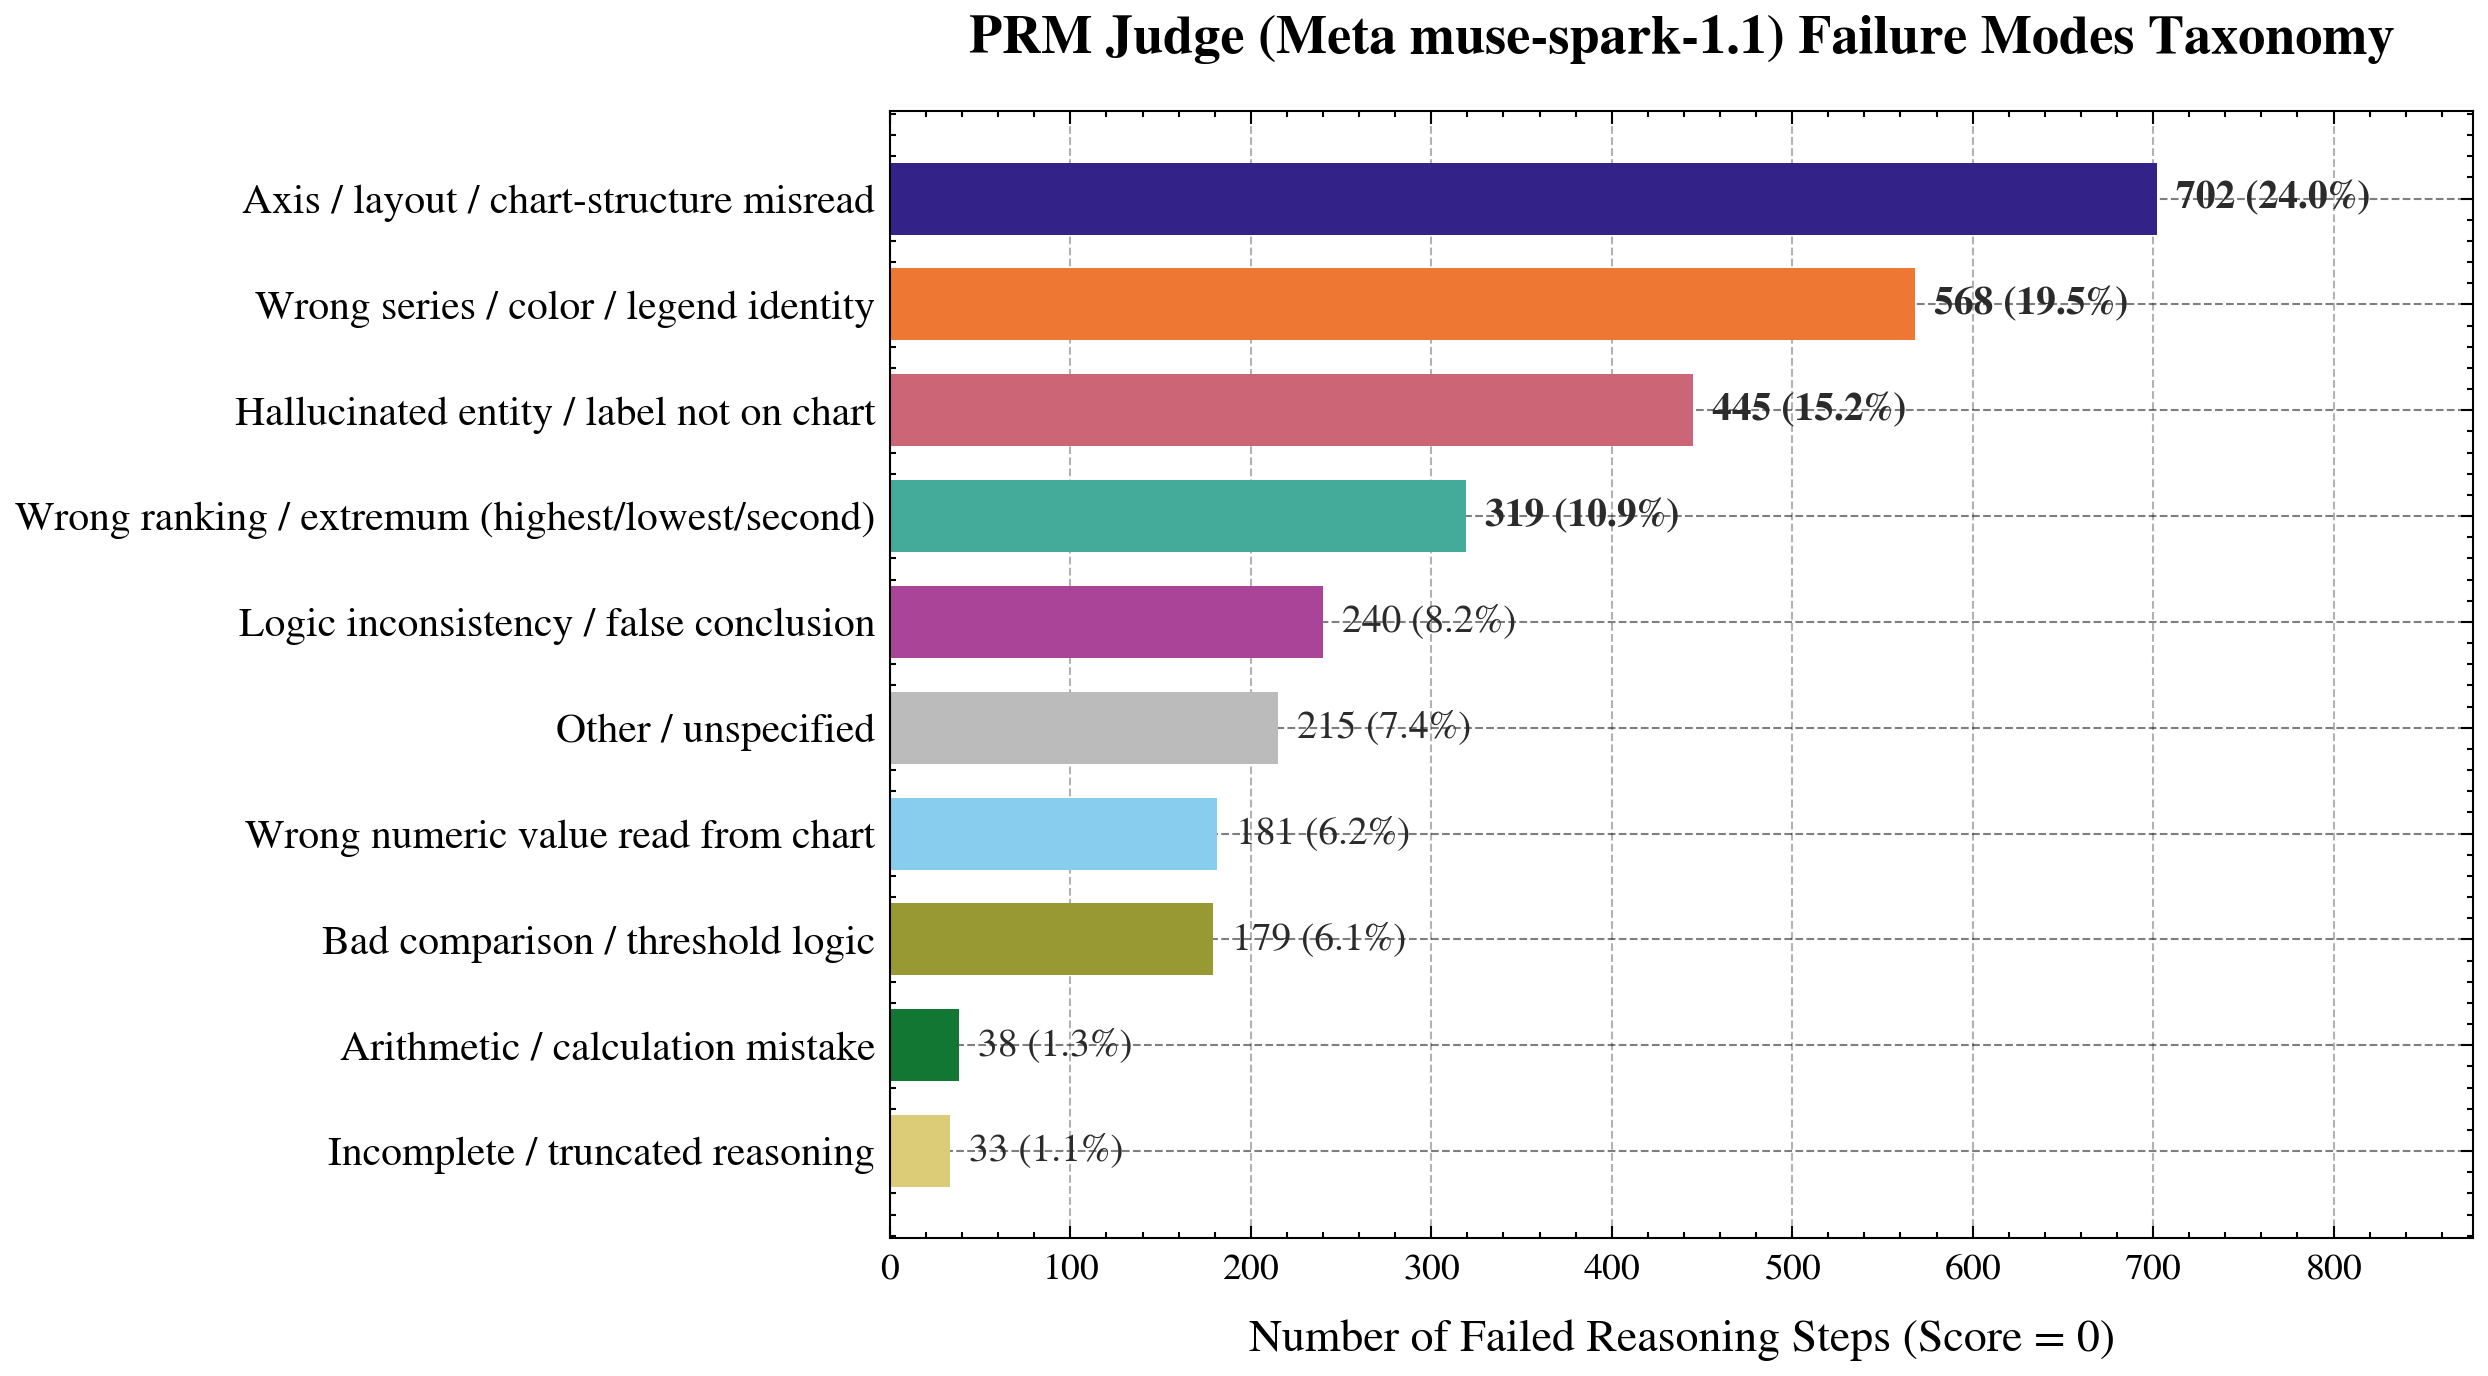
\includegraphics[width=\columnwidth]{../charts/report_selected/judge_01_error_taxonomy.png}
  \caption{\textbf{Distribution of 2,920 Refuted Reasoning Steps.} Visual grounding failures (axis misreads at 24.0\% and series confusion at 19.5\%) account for 43.5\% of all errors, whereas pure arithmetic mistakes account for only 1.3\%.}
  \label{fig:taxonomy_dist}
\end{figure}

To understand why the model fails, we analyze the natural language critique texts written by the judge across all 2,920 failed steps ($s_t = 0$). We categorize these critiques into a 9-category taxonomy using keyword matching and semantic clustering (see Table~\ref{tab:appendix_error_taxonomy} in Appendix~\ref{sec:appendix_diagnostics} for diagnostic keywords and critique excerpts). Figure~\ref{fig:taxonomy_dist} shows the overall distribution, while Figure~\ref{fig:error_by_step_depth} (in Appendix~\ref{sec:appendix_diagnostics}) details how error modes evolve across step depth.

\textbf{Perception vs. Arithmetic:} A central question in multimodal chart reasoning is whether models fail due to bad math or bad vision. Our empirical taxonomy gives a clear answer: failures are overwhelmingly perceptual. Axis and layout misreadings account for 24.0\% of all errors ($N=702$), while series and legend confusions make up 19.5\% ($N=568$). Together, pure visual grounding errors represent \textbf{43.5\%} ($N=1,270$) of all failed steps. 

In sharp contrast, pure arithmetic mistakes account for only \textbf{1.3\%} ($N=38$), or about 1 in every 77 errors. The model's computational logic is sound; its visual perception is the bottleneck. The model knows how to add, subtract, and compare numbers. However, it misreads logarithmic scales as linear (estimating 40 instead of 10), swaps line colors in crowded legends, or overlooks multi-panel subplot layouts. Once the initial numbers are read incorrectly, subsequent calculations cannot fix the error.

\textbf{Temporal Shift Across Steps:} As detailed in Figure~\ref{fig:error_by_step_depth} (Appendix~\ref{sec:appendix_diagnostics}), error types change as reasoning progresses. At Step 0, \textbf{78.5\%} of all errors are axis or layout misreads. In the opening step, the model tries to locate the right subplot and parse the axes. When this initial grounding fails, the remaining chain is corrupted. In Steps 2 through 4, errors shift from axis reading to comparative and logical mistakes: entity hallucinations (15.2\%), incorrect rankings or extrema (10.9\%), and logical contradictions (8.2\%). Downstream steps appear to suffer from broken logic, but they are actually operating on corrupted visual premises.

\subsection{Alignment Benchmark on Held-Out Reasoning}
\label{subsec:alignment_benchmark}

\begin{table*}[t]
\centering
\footnotesize
\setlength{\tabcolsep}{3.2pt}
\begin{tabular}{llccccccc}
\toprule
\textbf{Model} & \textbf{Supervision} & \textbf{EM Acc.} & \textbf{Token} & \textbf{Str+Acc} & \textbf{Recall} & \textbf{Struct} & \textbf{Preamb} & \textbf{Wrong} \\
\midrule
\texttt{Qwen2.5-VL-3B} & Base Instruct & 26.0\% & 28.0\% & 26.0\% & 63.0\% & 96.8\% & 7.0\% & 37.0\% \\
SFT & Gold Traces & 23.0\% & 28.0\% & 28.0\% & 57.0\% & \textbf{100.0\%} & \textbf{0.0\%} & 43.0\% \\
\textbf{Full DPO} & Chosen vs.\ Rej. & \textbf{29.0\%} & \textbf{30.0\%} & \textbf{29.0\%} & 51.0\% & 97.2\% & 5.0\% & 49.0\% \\
Step-DPO & Prefix-Masked & 25.0\% & 25.0\% & 16.0\% & 64.0\% & 67.6\% & 57.0\% & 36.0\% \\
KTO & Unpaired & 26.0\% & 29.0\% & 0.0\% & \textbf{66.0\%} & 21.2\% & 99.0\% & \textbf{30.0\%} \\
SFT$\rightarrow$DPO & Two-Stage & 22.0\% & 25.0\% & 25.0\% & 47.0\% & 97.8\% & \textbf{0.0\%} & 53.0\% \\
\midrule
\multicolumn{9}{l}{\textit{Specialist \& Reference-Free Extensions:}} \\
\texttt{ChartGemma} (3B) & Specialist & 27.0\% & 27.0\% & -- & -- & -- & -- & -- \\
SimPO & Ref.-Free & 26.0\% & 27.0\% & 26.0\% & -- & 95.0\% & 6.0\% & 40.0\% \\
Pareto-DPO & Multi-Filter & 30.0\% & 31.0\% & 30.0\% & -- & 97.0\% & 4.0\% & 46.0\% \\
\bottomrule
\end{tabular}
\caption{\textbf{Main Holdout Benchmark Evaluation on CharXiv ($N=100$).} EM Acc.\ is official exact-match accuracy; Token is normalized token match; Str+Acc is format-compliant and correct; Recall measures whether the ground truth is mentioned in text; Struct is structural compliance ($0$--$100$\%); Preamb is preamble penalty rate; Wrong is wrong committed answers (hallucination proxy).}
\label{tab:main_benchmark}
\end{table*}

We evaluate all aligned models on the held-out test split of 100 CharXiv reasoning problems. Table~\ref{tab:main_benchmark} reports performance across all seven alignment paradigms alongside a specialist baseline. We evaluate official exact-match accuracy (EM Acc.), normalized token match (Token), format-compliant accuracy (Str+Acc), ground-truth recall in text (Recall), structural compliance (Struct), conversational preamble penalty (Preamb), and committed wrong answer rate (Wrong).

\textbf{Pareto-DPO Is the Best System, Full DPO a Close Second:} Pareto-dominance-filtered DPO (\S\ref{subsec:dynamic_prm}) reaches the highest exact-match accuracy at \textbf{30.0\%} and the highest token match at \textbf{31.0\%}, outperforming the unaligned base model (26.0\%) by +4.0 percentage points. Full-sequence DPO is a close second at 29.0\% (+3.0 pp), trained on the same 134-pair budget but with single-scalar chosen/rejected selection rather than 9-dimensional dominance filtering. The gap between them (1.0 pp) is not statistically significant on $N=100$. Both results point to the same underlying claim: full-trajectory preference optimization, rather than format cloning, is what moves accuracy in this regime. Both models achieve near-identical, near-perfect structural compliance (97.0--97.2\%), so neither wins by sacrificing format for accuracy.

\textbf{The SFT Underperformance Paradox:} Supervised fine-tuning on 70 verified gold traces yields an exact-match accuracy of only \textbf{23.0\%}, falling 3.0 percentage points below the unaligned base model. Although SFT trains on human- and judge-approved demonstrations, it provides no negative feedback. In chart reasoning, knowing what not to read (such as distinguishing a dashed trend line from a solid confidence bound) is just as critical as seeing correct examples. SFT encourages rigid template memorization rather than adaptable visual grounding. Reference-free SimPO, trained on the same pairs as Full DPO but without a KL term against the reference policy, lands close to base (26.0\%): its tail preference accuracy during training was only 51.5\%, barely above chance, indicating 134 pairs at one epoch is not enough signal for this objective to reliably learn which trajectory to prefer.

\textbf{Step-DPO and KTO:} Suffix Step-DPO achieves \textbf{25.0\%} exact match. While Step-DPO focuses preference loss on the first divergent step, masking the shared prefix degrades the model's global sequence coherence, leading to formatting penalties. Unpaired KTO matches the base model at \textbf{26.0\%} exact match (29.0\% token match), but suffers from severe formatting collapse, as discussed below. Finally, two-stage SFT$\rightarrow$DPO achieves only \textbf{22.0\%} accuracy, showing that the inductive bias introduced during SFT warm-up hurts subsequent preference optimization.

\textbf{Validating the Small-Data Alignment Hypothesis:} These results answer our core research question. Aligning a 3B vision-language model does not require tens of thousands of expensive annotations. By using a multimodal judge to curate 134 clean, contrastive preference pairs, full-sequence DPO achieves a measurable +3.0 pp gain under a strict 16GB VRAM budget on Kaggle, and filtering those same pairs by Pareto dominance across a 9-dimensional failure profile (\S\ref{subsec:dynamic_prm}) pushes this further to +4.0 pp, CharXiv's best result.

\subsection{The Accuracy--Structure Trade-Off and Error Modes}
\label{subsec:accuracy_structure_tradeoff}

\begin{figure}[t]
  \centering
  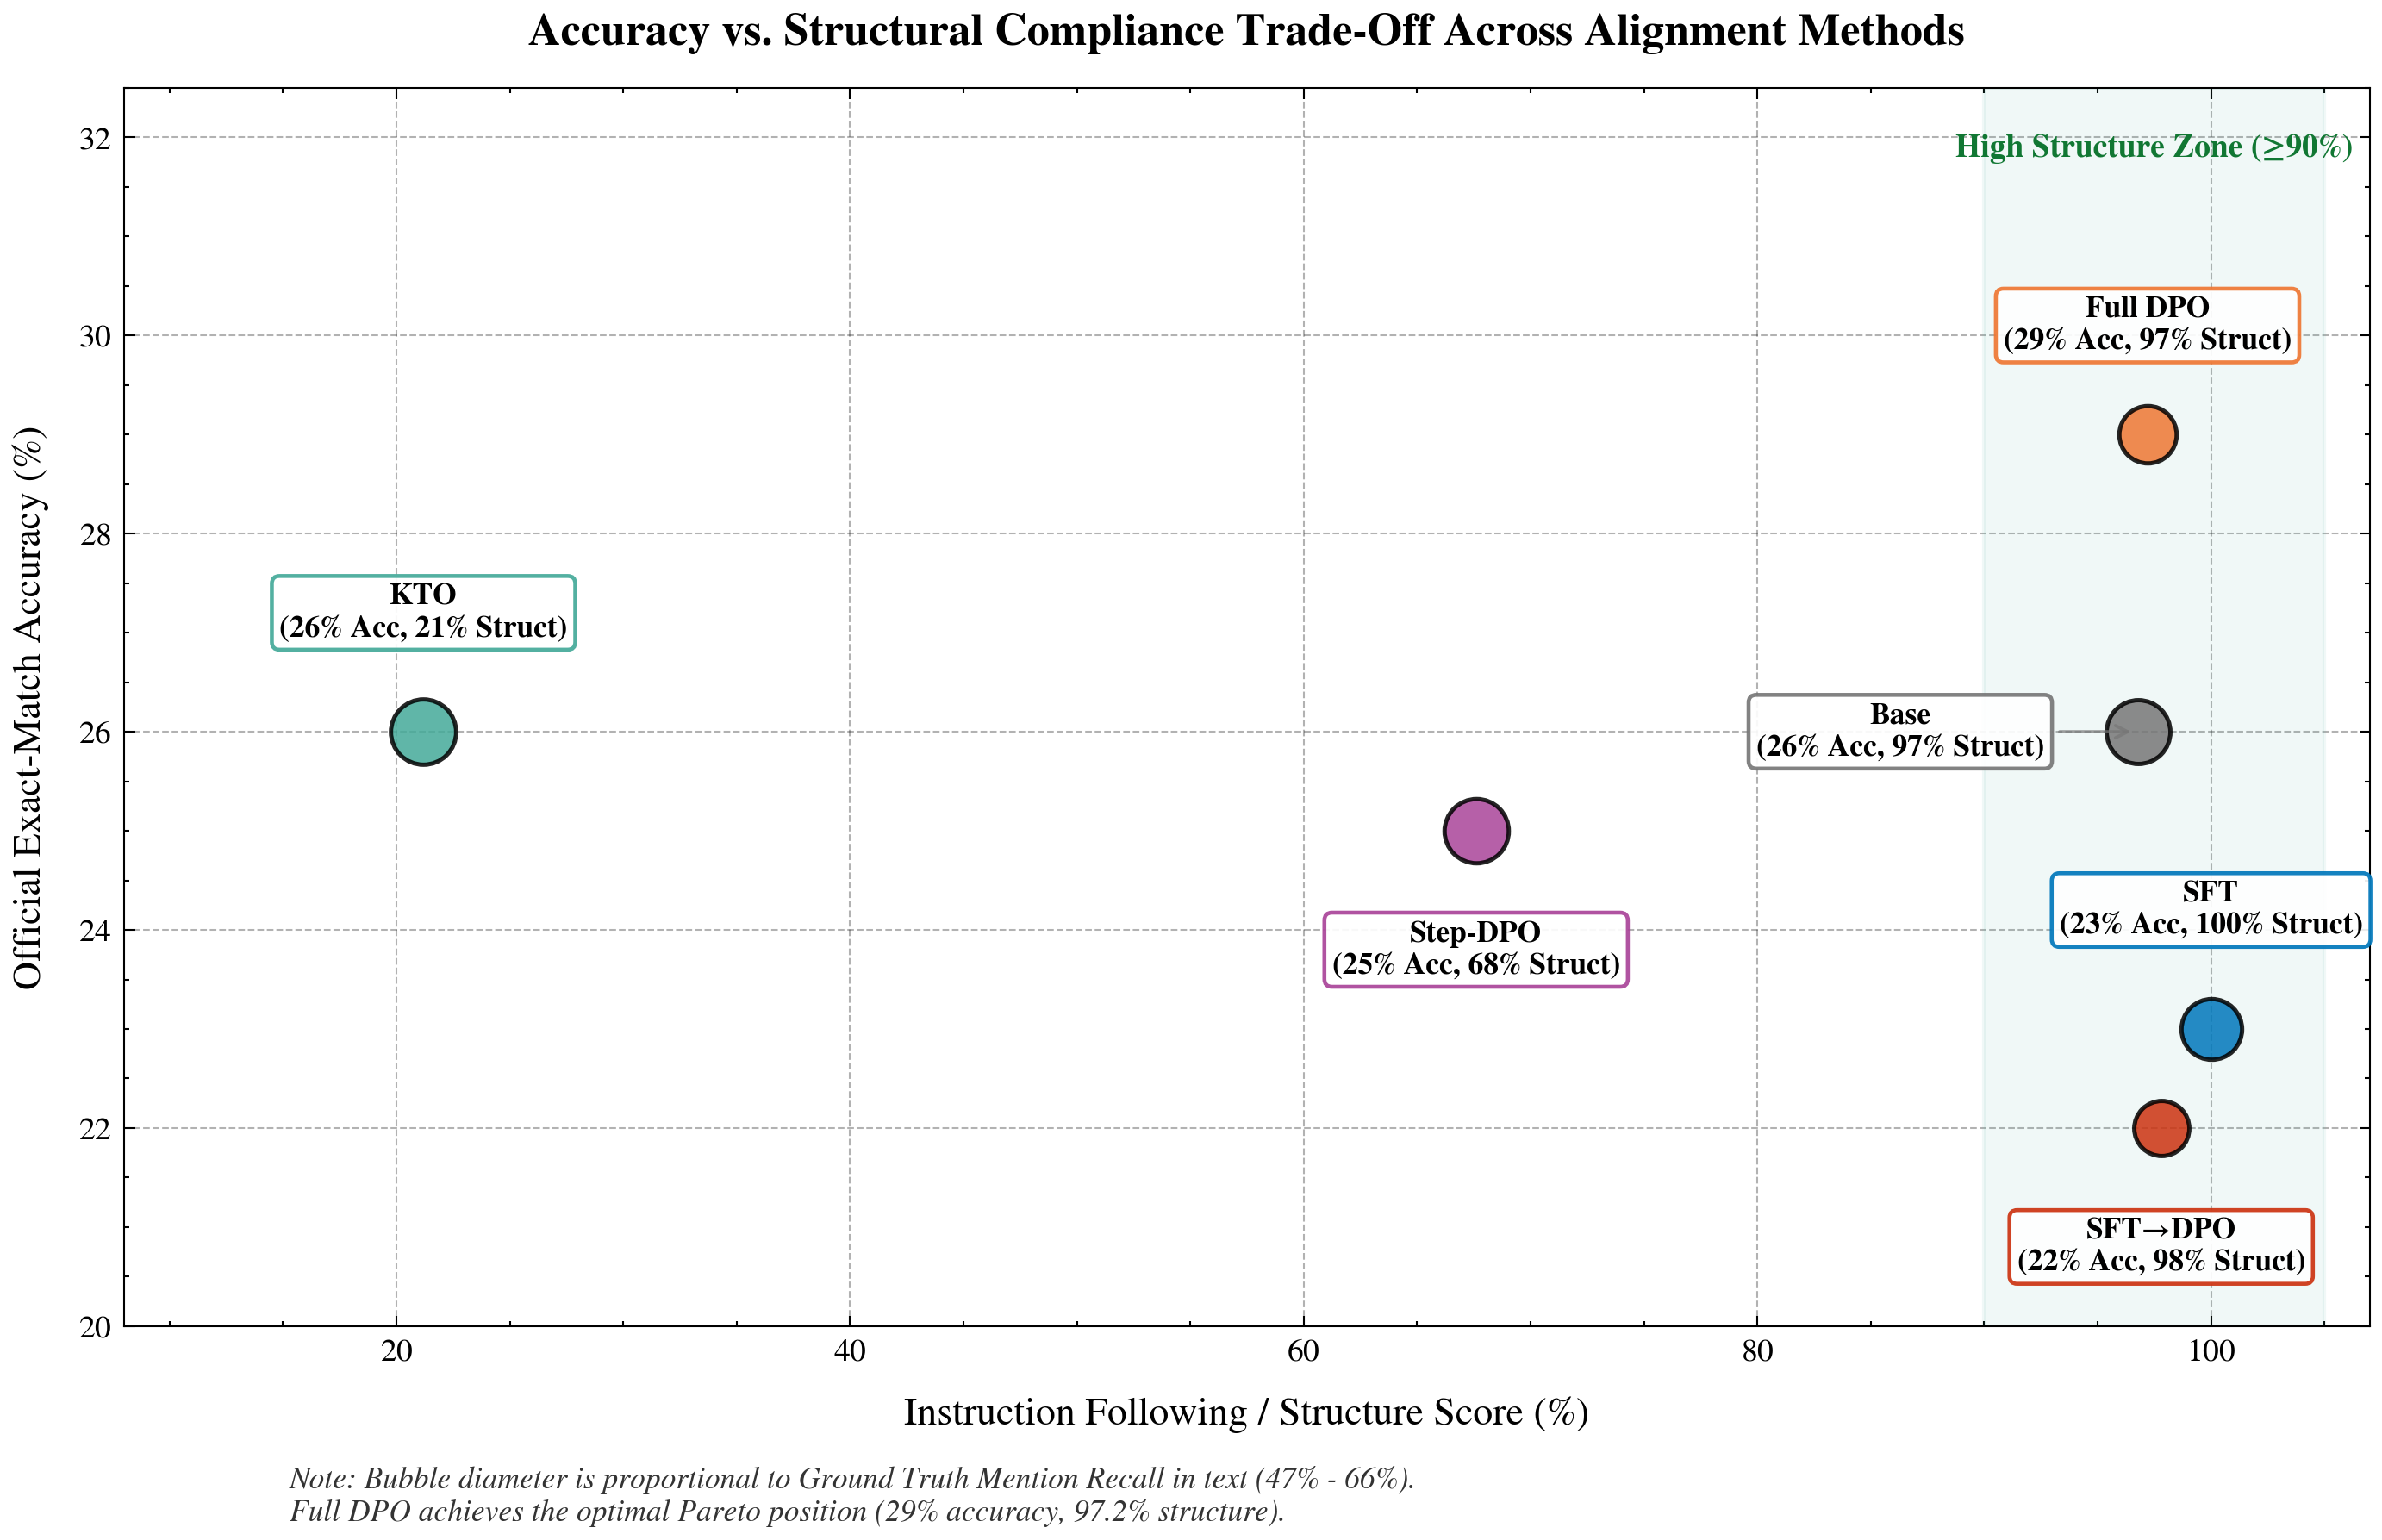
\includegraphics[width=\columnwidth]{../charts/report_selected/results_08_accuracy_vs_structure_tradeoff.png}
  \caption{\textbf{Accuracy vs. Structure Pareto Frontier.} Bubble diameter is proportional to ground-truth mention recall in prose (47\%--66\%). Full DPO achieves the best balance (29.0\% accuracy, 97.2\% structure). SFT attains 100\% structure at lower accuracy (23.0\%). KTO yields highest latent recall (66.0\%) but collapses structurally (21.2\%).}
  \label{fig:pareto_frontier}
\end{figure}

Standard benchmarks often hide how alignment alters instruction-following behavior. Figure~\ref{fig:pareto_frontier} plots official accuracy against structural compliance, where bubble sizes represent ground-truth recall in the model's text (whether the correct answer appears anywhere in the reasoning trace); full error-mode partitions into extracted correct, unextracted correct, partial mentions, and committed wrong answers are reported in Appendix~\ref{sec:appendix_diagnostics} (Figure~\ref{fig:error_modes}).

\textbf{The Pareto Frontier (Accuracy vs. Structure):}
Figure~\ref{fig:pareto_frontier} reveals a distinct Pareto frontier across the alignment paradigms:
\begin{itemize}[noitemsep,topsep=0pt]
    \item \textbf{SFT (Over-Constrained Rigidity):} SFT achieves a perfect 100.0\% structural compliance score with 0.0\% conversational preamble. Every trace begins with \texttt{Step 1:} and ends with a clean \texttt{Final Answer:}. However, this comes at the cost of reasoning flexibility (23.0\% accuracy). SFT fits the formatting prompt so rigidly that its capacity to deduce visual relationships is constrained.
    \item \textbf{Full DPO (The Pareto Optimum):} Full-trajectory DPO achieves the best overall trade-off: 29.0\% accuracy with 97.2\% structural compliance and only 5.0\% preamble penalty. It learns to avoid visual pitfalls while maintaining strict adherence to the output format.
    \item \textbf{KTO (Structural Collapse with High Latent Recall):} Unpaired KTO displays a striking contrast. Its structural compliance score collapses to 21.2\%, with 99.0\% of responses starting with conversational filler. Because KTO trains on unpaired positive and negative samples without pairwise comparison, it quickly forgets the strict format constraints. Yet, KTO achieves the highest ground-truth recall in prose at \textbf{66.0\%} (the largest bubble in Figure~\ref{fig:pareto_frontier}). KTO often names the correct numeric value in its reasoning, but fails to isolate it under the \texttt{Final Answer:} tag, leading to an official score of only 26.0\%.
    \item \textbf{Step-DPO (Format Drift):} Suffix Step-DPO achieves 67.6\% structure compliance but suffers a 57.0\% preamble penalty. Because its loss is calculated strictly on suffixes, the policy loses conditioning on the initial \texttt{Step 1:} instruction.
\end{itemize}

\textbf{Error Modes and Hallucination Proxy:}
Analyzing error-mode distributions (Figure~\ref{fig:error_modes}, Appendix~\ref{sec:appendix_diagnostics}), an important observation is the rate of \textit{committed wrong answers}---where the model outputs an incorrect final prediction without ever mentioning the true value in its reasoning.

Models with high structural discipline exhibit higher committed hallucination rates: SFT commits wrong answers in 43.0\% of cases, Full DPO in 49.0\%, and SFT$\rightarrow$DPO in 53.0\%. Because these models are strictly trained to produce a definite \texttt{Final Answer:}, they cannot express uncertainty. When their visual grounding fails, they commit decisively to a hallucinated number. By contrast, KTO has the lowest committed wrong rate (30.0\%) because its conversational explanations explore multiple possibilities, often mentioning the ground truth even when the final tag is missing.

\subsection{Cross-Dataset Generalization: ChartQA Holdout}
\label{subsec:chartqa_generalization}

The results above establish what works on CharXiv. A separate question is whether any of it is specific to CharXiv: a reward tree distilled from one benchmark's failure language could easily be overfit to that benchmark's visual style or question phrasing, and a pair-selection method that wins by 1.0 pp on $N=100$ could easily be noise. We test both concerns directly by rebuilding the entire pipeline, rollout generation, reward scoring, preference curation, and training, on a second, disjoint benchmark, \textbf{ChartQA} \citep{masry2022chartqa}, reusing the reward tree of \S\ref{subsec:dynamic_prm} unmodified: no retuning, no new criteria, no new judge calls to rebuild it. The reward tree's scoring itself runs on \texttt{gemini-3.5-flash-lite} rather than \texttt{muse-spark-1.1}, the model behind the binary step judge of \S\ref{subsec:prm_judge}; we switched for free-tier API access, not judge quality, and both CharXiv's and ChartQA's dynamic scores come from this same Gemini judge, so the cross-dataset comparison in this section is not confounded by a mid-experiment model change.

We sample 150 human-authored, non-yes/no reasoning questions from ChartQA's official test split as a training pool and hold out 30 more for evaluation, mirroring the same reasoning/descriptive distinction CharXiv itself uses: ChartQA's human-authored questions require genuine chart reading, while its machine-generated split is templated, closer to CharXiv's excluded descriptive questions. All seven alignment methods are retrained from scratch on this pool with the same hyperparameters as their CharXiv counterparts (Table~\ref{tab:training_setup}) and evaluated on the 30-question holdout with the same metrics as Table~\ref{tab:main_benchmark}.

\begin{table*}[t]
\centering
\footnotesize
\setlength{\tabcolsep}{3.2pt}
\begin{tabular}{llccccccc}
\toprule
\textbf{Model} & \textbf{Supervision} & \textbf{EM Acc.} & \textbf{Token} & \textbf{Str+Acc} & \textbf{Recall} & \textbf{Struct} & \textbf{Preamb} & \textbf{Wrong} \\
\midrule
\texttt{Qwen2.5-VL-3B} & Base Instruct & 43.3\% & 60.0\% & 60.0\% & 66.7\% & \textbf{100.0\%} & \textbf{0.0\%} & 33.3\% \\
SFT & Gold Traces & 43.3\% & 56.7\% & 56.7\% & 63.3\% & \textbf{100.0\%} & \textbf{0.0\%} & 36.7\% \\
Full DPO & Chosen vs.\ Rej. & 40.0\% & 50.0\% & 26.7\% & 63.3\% & 73.3\% & 46.7\% & 33.3\% \\
Step-DPO & Prefix-Masked & 36.7\% & 46.7\% & 20.0\% & 63.3\% & 59.3\% & 56.7\% & 33.3\% \\
KTO & Unpaired & 36.7\% & 50.0\% & 0.0\% & 66.7\% & 32.7\% & 86.7\% & \textbf{23.3\%} \\
SFT$\rightarrow$DPO & Two-Stage & 40.0\% & 53.3\% & 53.3\% & 60.0\% & 98.7\% & \textbf{0.0\%} & 40.0\% \\
\midrule
\multicolumn{9}{l}{\textit{Reference-Free and Multi-Filter Extensions:}} \\
SimPO & Ref.-Free & 43.3\% & 60.0\% & 60.0\% & 66.7\% & \textbf{100.0\%} & \textbf{0.0\%} & 33.3\% \\
\textbf{Pareto-DPO} & Multi-Filter & \textbf{60.0\%} & \textbf{73.3\%} & \textbf{73.3\%} & \textbf{73.3\%} & \textbf{100.0\%} & \textbf{0.0\%} & 26.7\% \\
\bottomrule
\end{tabular}
\caption{\textbf{Cross-Dataset Holdout Evaluation on ChartQA ($N=30$).} Same seven methods, same hyperparameters, same metrics as Table~\ref{tab:main_benchmark}, retrained from scratch on an independently sampled ChartQA pool. Pareto-DPO leads on every column except Wrong.}
\label{tab:chartqa_benchmark}
\end{table*}

\begin{figure}[t]
  \centering
  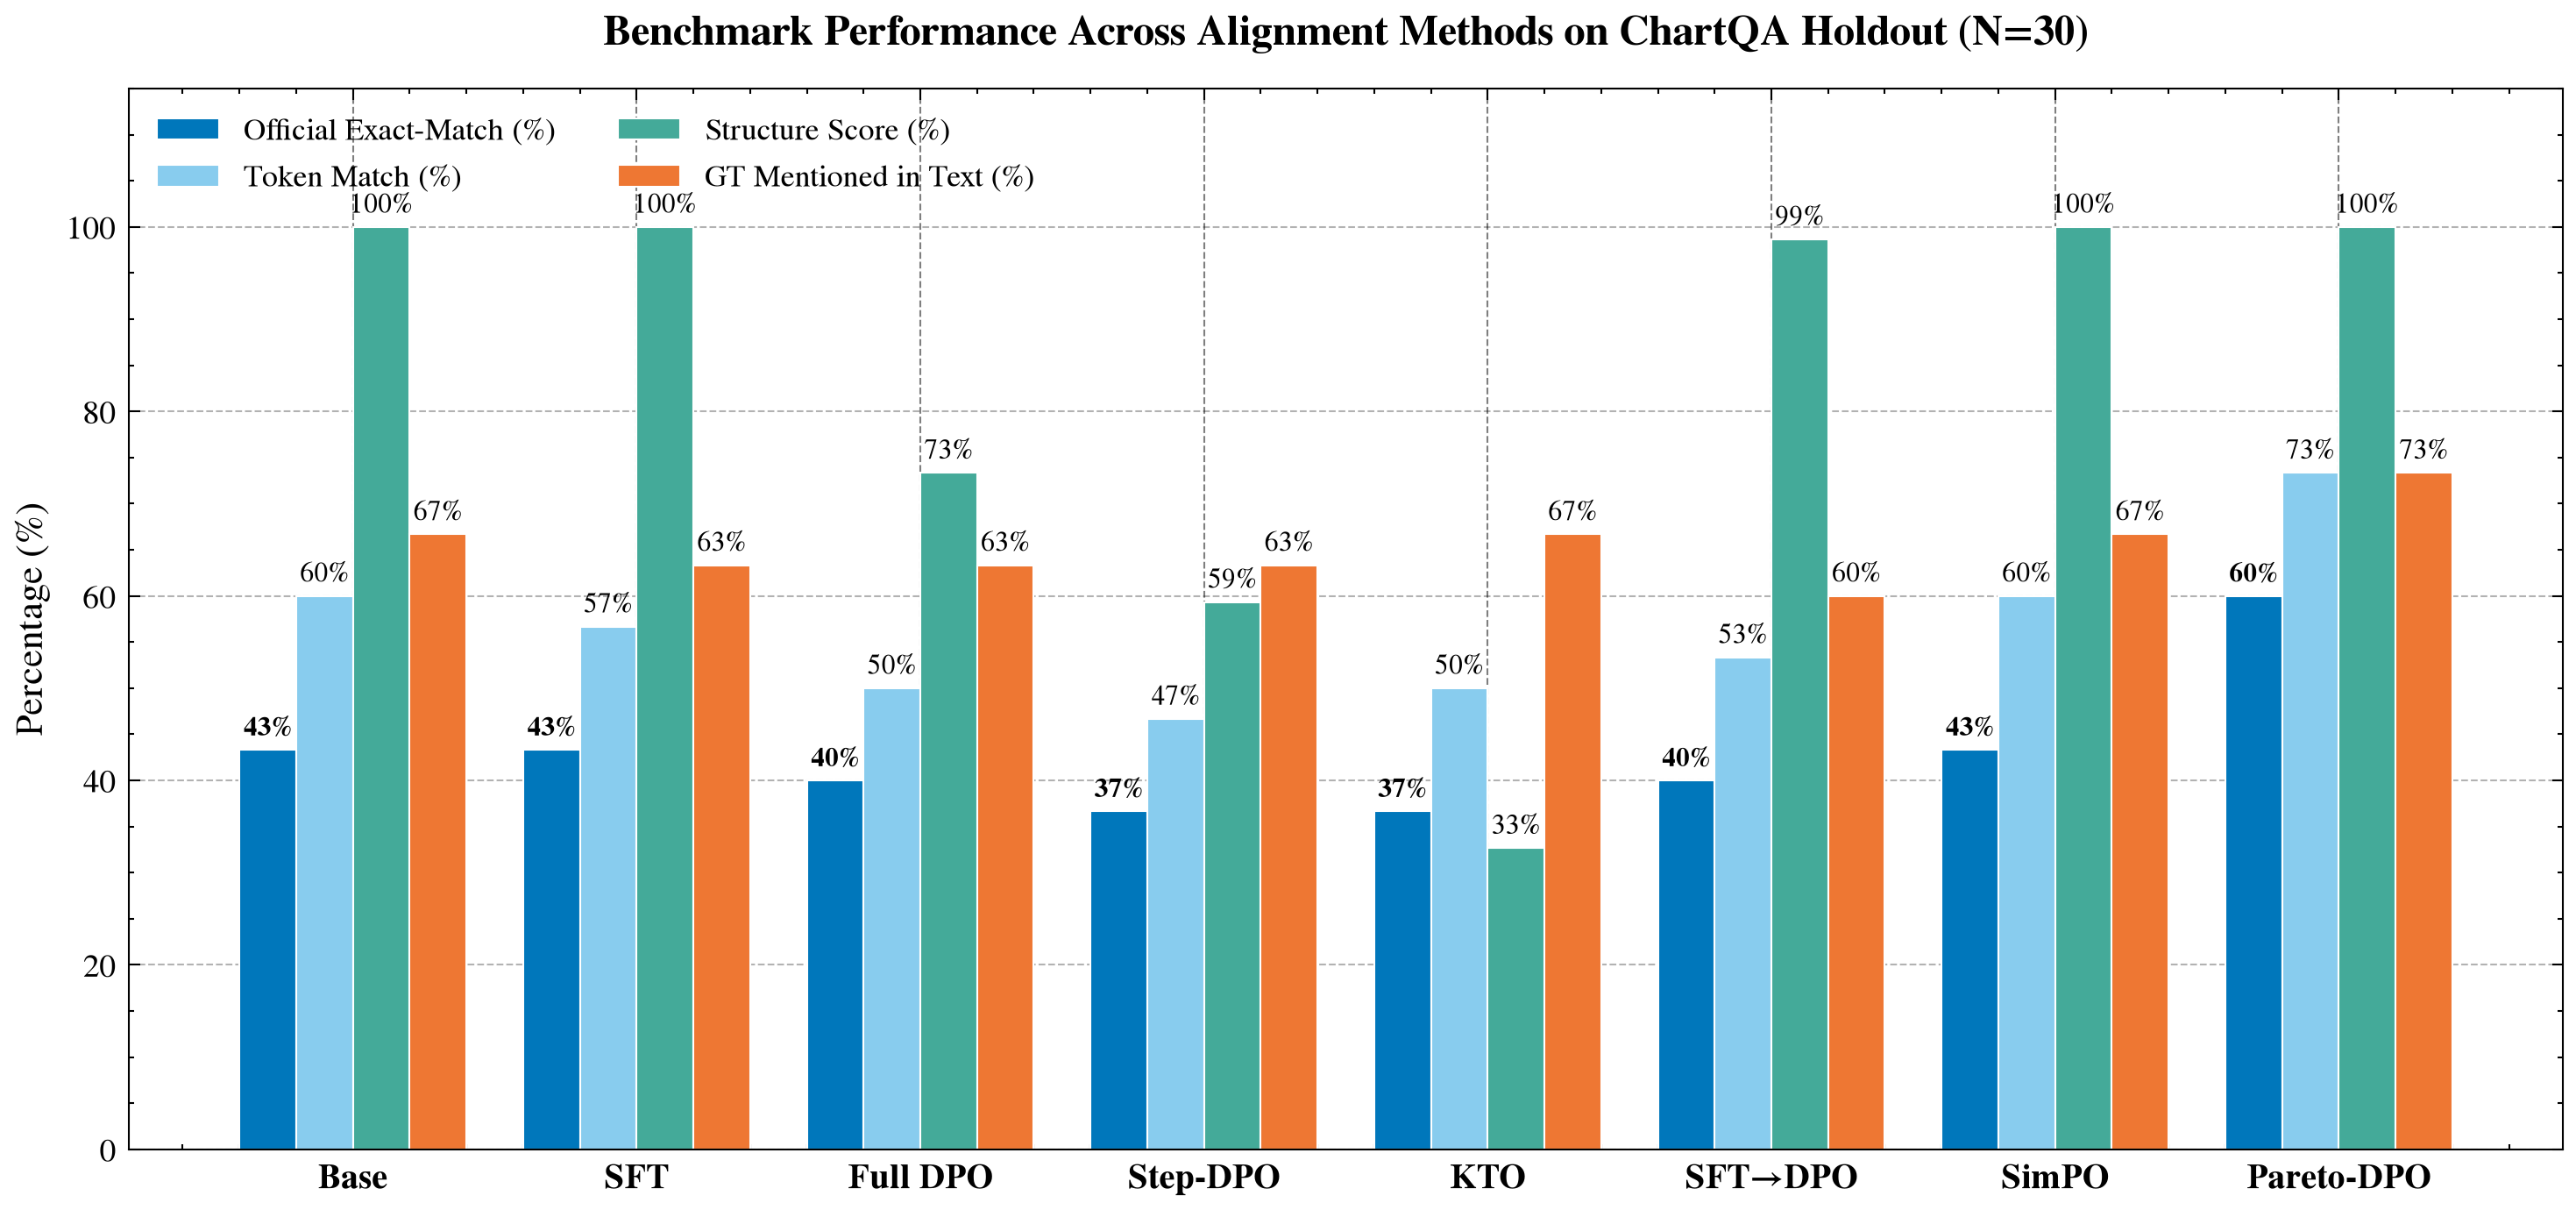
\includegraphics[width=\columnwidth]{../charts/chartqa/chartqa_01_overall_comparison.png}
  \caption{\textbf{ChartQA Holdout Benchmark ($N=30$).} Pareto-DPO leads on exact-match, token match, and structure score simultaneously, the same pattern of a single method winning on every axis that Table~\ref{tab:chartqa_benchmark} shows numerically.}
  \label{fig:chartqa_overall}
\end{figure}

\begin{figure}[t]
  \centering
  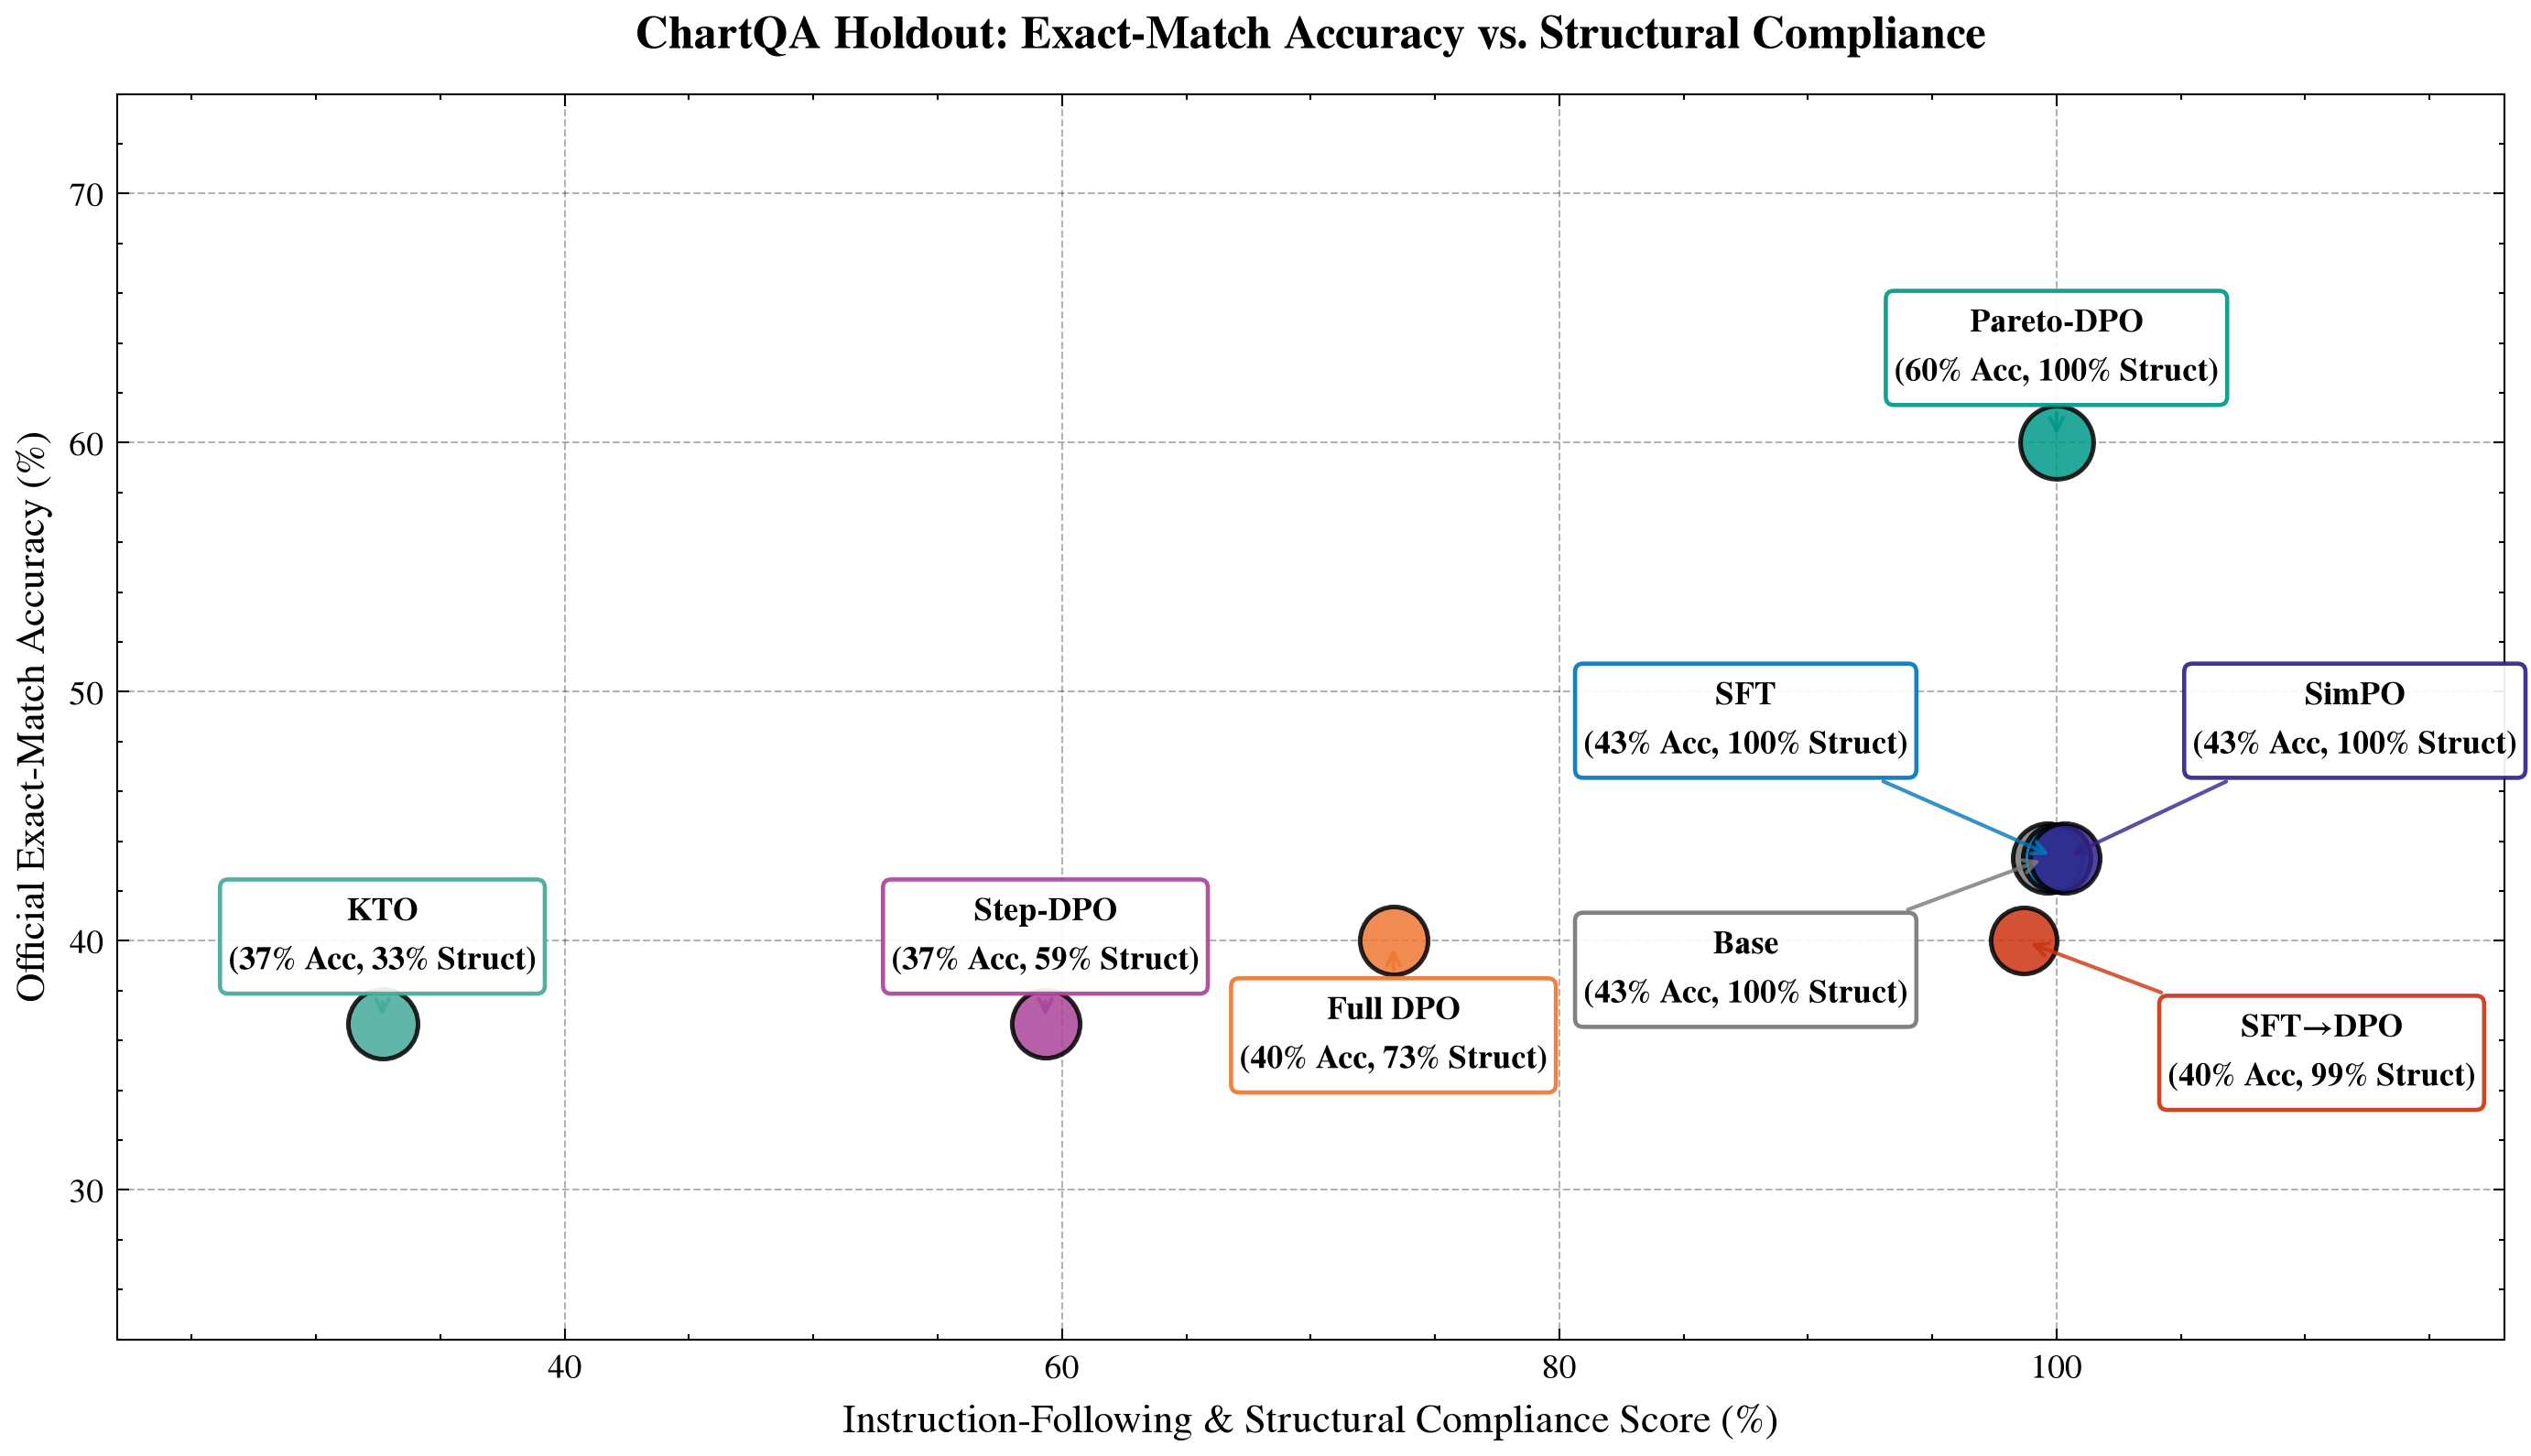
\includegraphics[width=\columnwidth]{../charts/chartqa/chartqa_03_accuracy_vs_structure_tradeoff.png}
  \caption{\textbf{ChartQA Accuracy vs.\ Structure Trade-Off.} Compare with Figure~\ref{fig:pareto_frontier}: on CharXiv, the trade-off separates methods along a frontier: on ChartQA, Pareto-DPO dominates outright, decisively ahead on accuracy while matching the highest structure score.}
  \label{fig:chartqa_tradeoff}
\end{figure}

\textbf{Pareto-DPO Wins Decisively:} Table~\ref{tab:chartqa_benchmark} and Figure~\ref{fig:chartqa_overall} show the same method that led on CharXiv (30.0\%) now leads on ChartQA by a much wider margin: \textbf{60.0\%} exact-match against a 43.3\% base, +16.7 percentage points, the largest gain of any method on either dataset. It also achieves the best token match (73.3\%), perfect structural compliance (100.0\%), and the highest ground-truth recall (73.3\%). Unlike on CharXiv, where Full DPO trailed by only 1.0 pp, the gap here is decisive (Figure~\ref{fig:chartqa_tradeoff}): Full DPO reaches only 40.0\%, tied with SFT$\rightarrow$DPO and 20 points behind. This comparison carries far less statistical power than CharXiv's $N=100$ holdout, however: at $N=30$, a single question flip moves exact-match by 3.3 pp, and a 5-question flip, plausible sampling noise at this scale, would move it by 16.7 pp, most of Pareto-DPO's entire margin over Full DPO.

\textbf{SFT and SimPO Tie Base:} Both SFT (43.3\%) and SimPO (43.3\%) match the base model exactly on ChartQA, echoing their CharXiv behavior (SFT $-3.0$ pp there, SimPO essentially tied at 26.0\%). SimPO's tail preference accuracy during training was 51.6\% on ChartQA, statistically indistinguishable from CharXiv's own 51.5\%, evidence this is a property of the reference-free objective at this pair count and epoch budget, not noise specific to either dataset.

\textbf{Step-DPO and KTO Reproduce Their CharXiv Collapse:} Both methods again show the largest structural degradation, and more severely than on CharXiv. Step-DPO's structure score drops to 59.3\% (vs.\ 67.6\% on CharXiv) with a 56.7\% preamble penalty. KTO collapses further, to 32.7\% structure and 0\% \texttt{Step 1:} starts, with 86.7\% of responses opening with conversational filler, worse than CharXiv's already-poor 21.2\%. KTO's collapse guard fired 110 times over 1,176 training steps on ChartQA (\S\ref{subsec:dynamic_prm}), the same generative-collapse tendency observed on CharXiv and unchanged by the switch in dataset. KTO does retain the lowest wrong-committed rate on ChartQA (23.3\%), the same trade-off seen on CharXiv: its conversational answers hedge rather than commit, at the cost of format.

\textbf{Training Signal Does Not Predict Holdout Accuracy:} SFT$\rightarrow$DPO reaches the highest per-step preference accuracy of any DPO-family method during ChartQA training (76.6\%), yet lands at only 40.0\% on the holdout, tied with Full DPO and far behind Pareto-DPO's 60.0\% despite Pareto-DPO's more modest 60.9\% training accuracy. The model that most reliably prefers the chosen response during training is not the model most likely to answer correctly after training. What distinguishes Pareto-DPO is the construction of its pairs, built to rule out ambiguous trade-offs a single scalar cannot see, rather than any advantage in how easily its preference signal is fit.

\textbf{What Transfers:} Taken together with the reward tree's transfer in \S\ref{subsec:dynamic_prm}, these results separate two claims that could otherwise be conflated. The dynamic judge transfers uneventfully: its criteria remain applicable, at undiminished density, to a chart source it never saw. Pareto-dominance pair selection transfers further than that: it is not merely applicable on ChartQA, it is the best-performing method there, by a wider margin than on CharXiv itself. The other six methods largely reproduce their CharXiv rank order and characteristic failure modes (KTO's collapse, Step-DPO's drift, SFT's rigidity), evidence that what we observe on CharXiv reflects properties of the methods and the small-data regime, not artifacts of one benchmark.

% Conclusions and Limitations will be added in subsequent steps
% \section{Conclusions}
% \label{sec:conclusions}
% \section*{Limitations}

% References
\clearpage
\nocite{*}
\bibliography{custom}

% Appendix
\clearpage
\appendix
\renewcommand{\thesection}{Appendix \Alph{section}}
\section{Full Alignment Objective Formulas}
\label{sec:appendix_objectives}

The main text (\S\ref{subsec:alignment_objectives}) gives the training data, hyperparameters, and a one-line description of each objective below; Full-Sequence DPO's loss (Equation~\ref{eq:dpo_loss}) remains in the main text since Pareto-DPO reuses it unchanged and every other objective here is defined relative to it.

\textbf{SFT} maximizes the log-likelihood of verified gold reasoning steps:
\begin{equation}
    \mathcal{L}_{\text{SFT}}(\theta) = -\mathbb{E}_{(x, y_w)} \sum_{t=1}^{|y_w|} \log \pi_\theta(y_{w,t} \mid x, y_{w,<t})
    \label{eq:sft_loss}
\end{equation}

\textbf{Suffix Step-DPO} applies the DPO loss only to the divergent suffix starting at the first point of disagreement $t^*$:
\begin{align}
    \mathcal{L}_{\text{Step-DPO}}(\theta) = -\mathbb{E} \Big[ \log \sigma \Big( & \beta \sum_{k \ge t^*} \log \tfrac{\pi_\theta(y_{w,k})}{\pi_{\text{ref}}(y_{w,k})} \nonumber \\
    {} - & \beta \sum_{k \ge t^*} \log \tfrac{\pi_\theta(y_{l,k})}{\pi_{\text{ref}}(y_{l,k})} \Big) \Big]
    \label{eq:stepdpo_loss}
\end{align}

\textbf{KTO} applies a prospect-theoretic utility function to unpaired desirable/undesirable completions:
\begin{equation}
    \mathcal{L}_{\text{KTO}}(\theta) = \mathbb{E}_{y} \left[ w(y) \left( 1 - v_\beta \left( \hat{r}_\theta(x, y) - z_{\text{ref}} \right) \right) \right]
    \label{eq:kto_loss}
\end{equation}
where $v_\beta(r) = \sigma(\beta r)$ for desirable outputs, $v_\beta(r) = \sigma(-\beta r)$ for undesirable outputs, and $z_{\text{ref}}$ is a running estimate of the implicit reward KL baseline.

\textbf{SimPO} replaces the reference-relative KL term with the policy's own length-normalized log-probability and a target margin $\gamma$:
\begin{align}
    \mathcal{L}_{\text{SimPO}}(\theta) = -\mathbb{E} \Big[ \log \sigma \Big( & \tfrac{\beta}{|y_w|} \log \pi_\theta(y_w \mid x) \nonumber \\
    {} - & \tfrac{\beta}{|y_l|} \log \pi_\theta(y_l \mid x) - \gamma \Big) \Big]
    \label{eq:simpo_loss}
\end{align}

\section{Supplementary Training and Diagnostic Visualizations}
\label{sec:appendix_diagnostics}

\begin{table*}[t]
\centering
\footnotesize
\setlength{\tabcolsep}{3.5pt}
\begin{tabular}{lcr p{3.2cm} p{5.2cm}}
\toprule
\textbf{Error Category} & \textbf{Count} & \textbf{Share} & \textbf{Diagnostic Keywords} & \textbf{Representative Judge Critique Excerpt} \\
\midrule
Axis / Layout Misread & $N=702$ & 24.0\% & \textit{axis, subplot, layout, horizontal, vertical} & ``Misreads the logarithmic y-axis scale as linear, estimating 40 instead of 10.'' \\
Wrong Series / Color & $N=568$ & 19.5\% & \textit{blue, line, red, legend, green, curve, orange} & ``Attributes the dashed orange curve to Baseline B, but legend associates it with Model A.'' \\
Hallucinated Entity & $N=445$ & 15.2\% & \textit{hallucinated, absent, not present, visible} & ``Refers to a third bar group for year 2020 which does not appear in the figure.'' \\
Wrong Ranking / Extremum & $N=319$ & 10.9\% & \textit{highest, lowest, largest, maximum, minimum} & ``Claims Method 1 achieves highest precision, but Method 3 is clearly higher.'' \\
Logic Inconsistency & $N=240$ & 8.2\% & \textit{contradicts, concludes, therefore, visual} & ``Correctly identifies coordinates 4.2 and 5.1, but falsely concludes 4.2 > 5.1.'' \\
Wrong Numeric Value & $N=181$ & 6.2\% & \textit{misreads, chart shows, near, false reading} & ``Reads point height as 0.65 when the marker aligns with the 0.50 gridline.'' \\
Bad Comparison / Logic & $N=179$ & 6.1\% & \textit{threshold, exceeds, comparison, logic} & ``Fails to evaluate whether the curve remains strictly above the margin.'' \\
Arithmetic Mistake & $N=38$ & 1.3\% & \textit{miscalculates, arithmetic, computation, sum} & ``Correctly extracts values 15 and 8, but computes the difference as 9.'' \\
Incomplete / Truncated & $N=33$ & 1.1\% & \textit{truncated, incomplete, cuts off, empty} & ``Generation terminates prematurely mid-sentence without a verifiable step.'' \\
Other / Unspecified & $N=215$ & 7.4\% & \textit{unspecified, error, incorrect} & ``Vague failure critique without explicit grounding attribution.'' \\
\midrule
\textbf{Perceptual Total} & $N=1,270$ & \textbf{43.5\%} & \multicolumn{2}{l}{\textit{Combined Axis Misread ($24.0\%$) and Series/Legend Identity ($19.5\%$)}} \\
\textbf{Arithmetic Total} & $N=38$ & \textbf{1.3\%} & \multicolumn{2}{l}{\textit{Pure calculation failure accounts for only $1$ in $77$ step errors}} \\
\bottomrule
\end{tabular}
\caption{\textbf{PRM Judge Error Taxonomy from 2,920 Refuted Reasoning Steps.} Categorized via priority-regex analysis over natural language critiques from \texttt{muse-spark-1.1}. Visual grounding (axes, series colors) forms the primary reasoning bottleneck, while arithmetic mistakes are rare.}
\label{tab:appendix_error_taxonomy}
\end{table*}

\begin{figure*}[t]
  \centering
  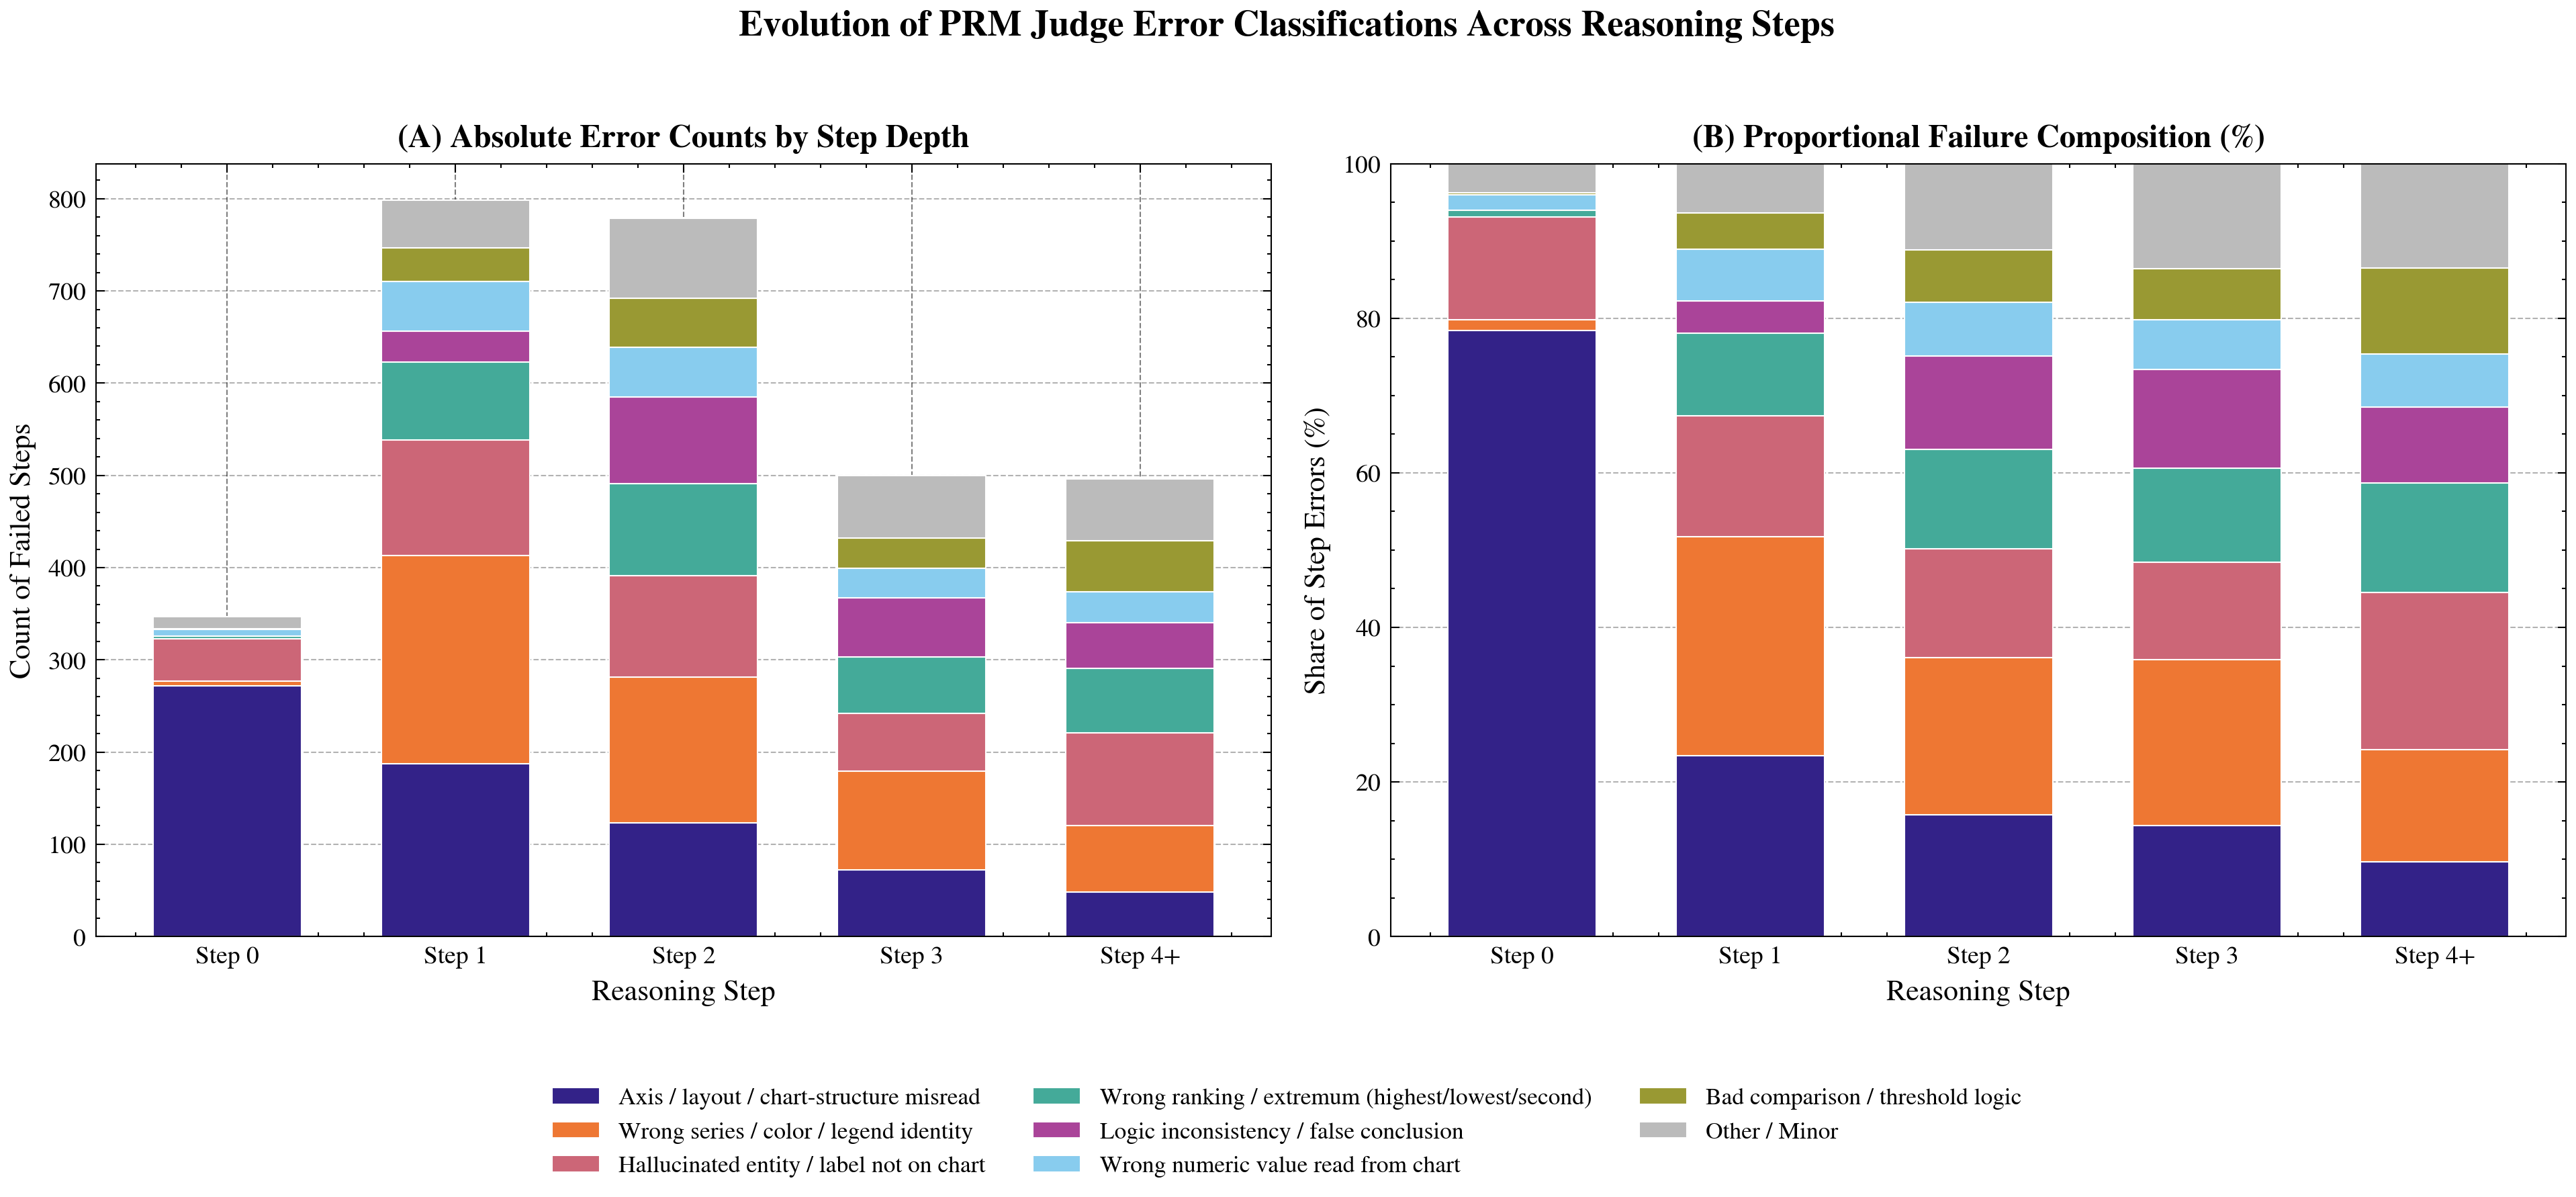
\includegraphics[width=0.98\textwidth]{../charts/report_selected/judge_02_error_by_step_depth.png}
  \caption{\textbf{Error Mode Composition Across Step Depth.} Detailed breakdown of 2,920 refuted reasoning steps evaluated by \texttt{muse-spark-1.1} across reasoning steps 0 to 4+. Step 0 is dominated by axis and layout misreads (78.5\%), which triggers cascading entity hallucinations and logical inconsistencies in downstream steps.}
  \label{fig:error_by_step_depth}
\end{figure*}

\begin{table}[t]
\centering
\footnotesize
\setlength{\tabcolsep}{3.5pt}
\begin{tabular}{lrr}
\toprule
\textbf{Trajectory Metric} & \textbf{Count} & \textbf{Share} \\
\midrule
CharXiv Reasoning Problems & 500 & 100.0\% \\
Evaluated Rollout Traces & 1,274 & 100.0\% \\
Mean Candidates / Question & 3.83 & -- \\
Total Judged Reasoning Steps & 4,947 & 100.0\% \\
\midrule
\textbf{Step Verification:} & & \\
-- Step Pass Rate ($\text{Score} = 1$) & 2,027 & 41.0\% \\
-- Step Failure Rate ($\text{Score} = 0$) & 2,920 & 59.0\% \\
\midrule
\textbf{Rollout Outcome:} & & \\
-- Fully Valid Rollouts (All steps $= 1$) & 154 & 12.1\% \\
-- Rollouts with $\ge 1$ Step Error & 1,120 & 87.9\% \\
Mean Steps per Rollout & 3.88 & -- \\
\midrule
\textbf{Failure Progression Dynamics:} & & \\
-- First Error at Step 0 & 347 & 31.0\% \\
-- First Error at Step 1 & 546 & 48.8\% \\
-- First Error at Step $\le 1$ Cumulative & 893 & \textbf{79.7\%} \\
-- Cascade: $P(S_{N+1}=0 \mid S_N=0)$ & 1,630 & \textbf{82.7\%} \\
-- Recovery: $P(S_{N+1}=1 \mid S_N=0)$ & 340 & 17.3\% \\
\bottomrule
\end{tabular}
\caption{\textbf{Reasoning Trajectory Statistics on CharXiv 500 Pool.} Over 79\% of trajectory errors begin within the first two steps. Once an error occurs, downstream steps fail 82.7\% of the time.}
\label{tab:trajectory_stats}
\end{table}

\begin{figure}[t]
  \centering
  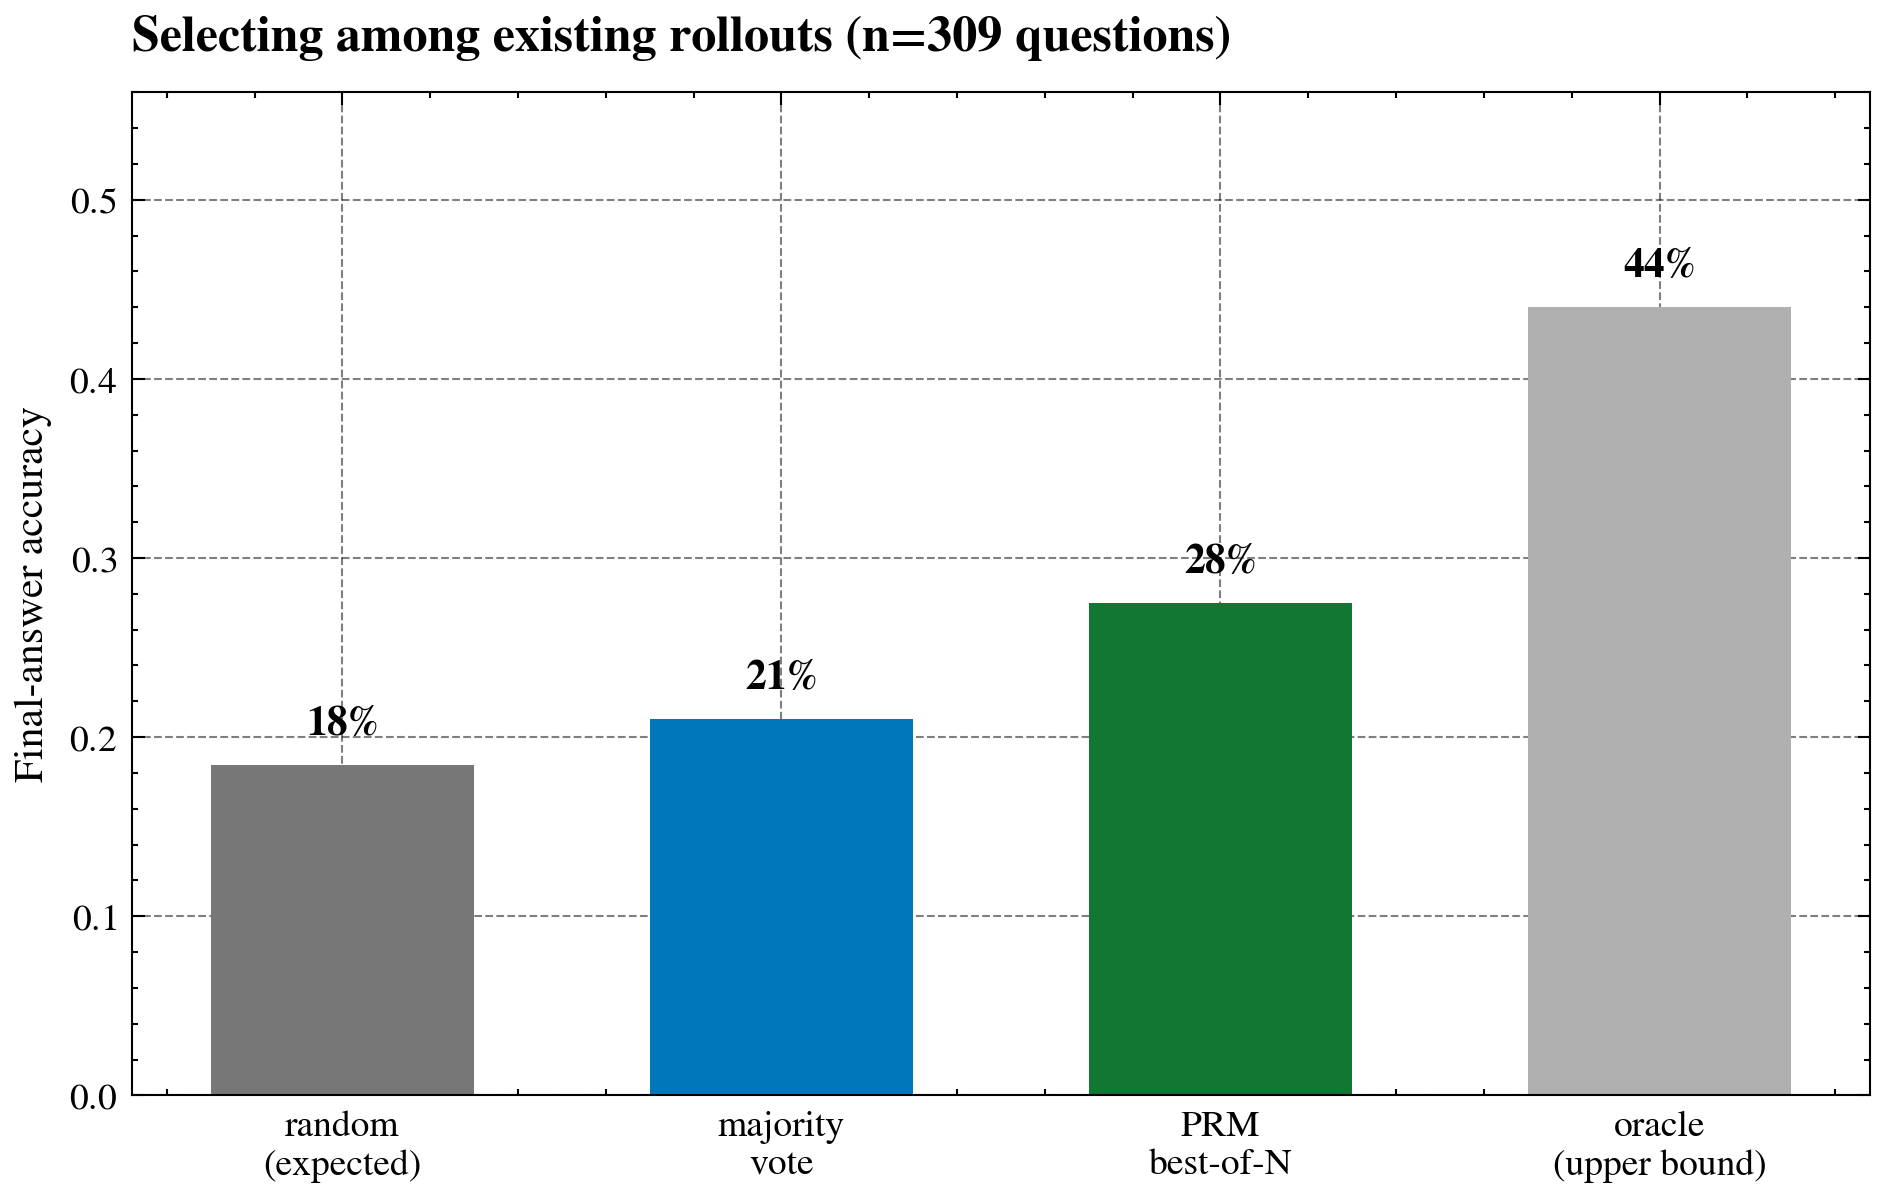
\includegraphics[width=\columnwidth]{../charts/report_selected/prm_best_of_n_accuracy.png}
  \caption{\textbf{Inference-Time PRM Verifier Accuracy.} Average step process reward selection (27.5\%) outperforms self-consistency majority voting (21.0\%) and random rollouts (18.4\%) across 309 multi-candidate questions.}
  \label{fig:prm_best_of_n}
\end{figure}

\begin{figure}[t]
  \centering
  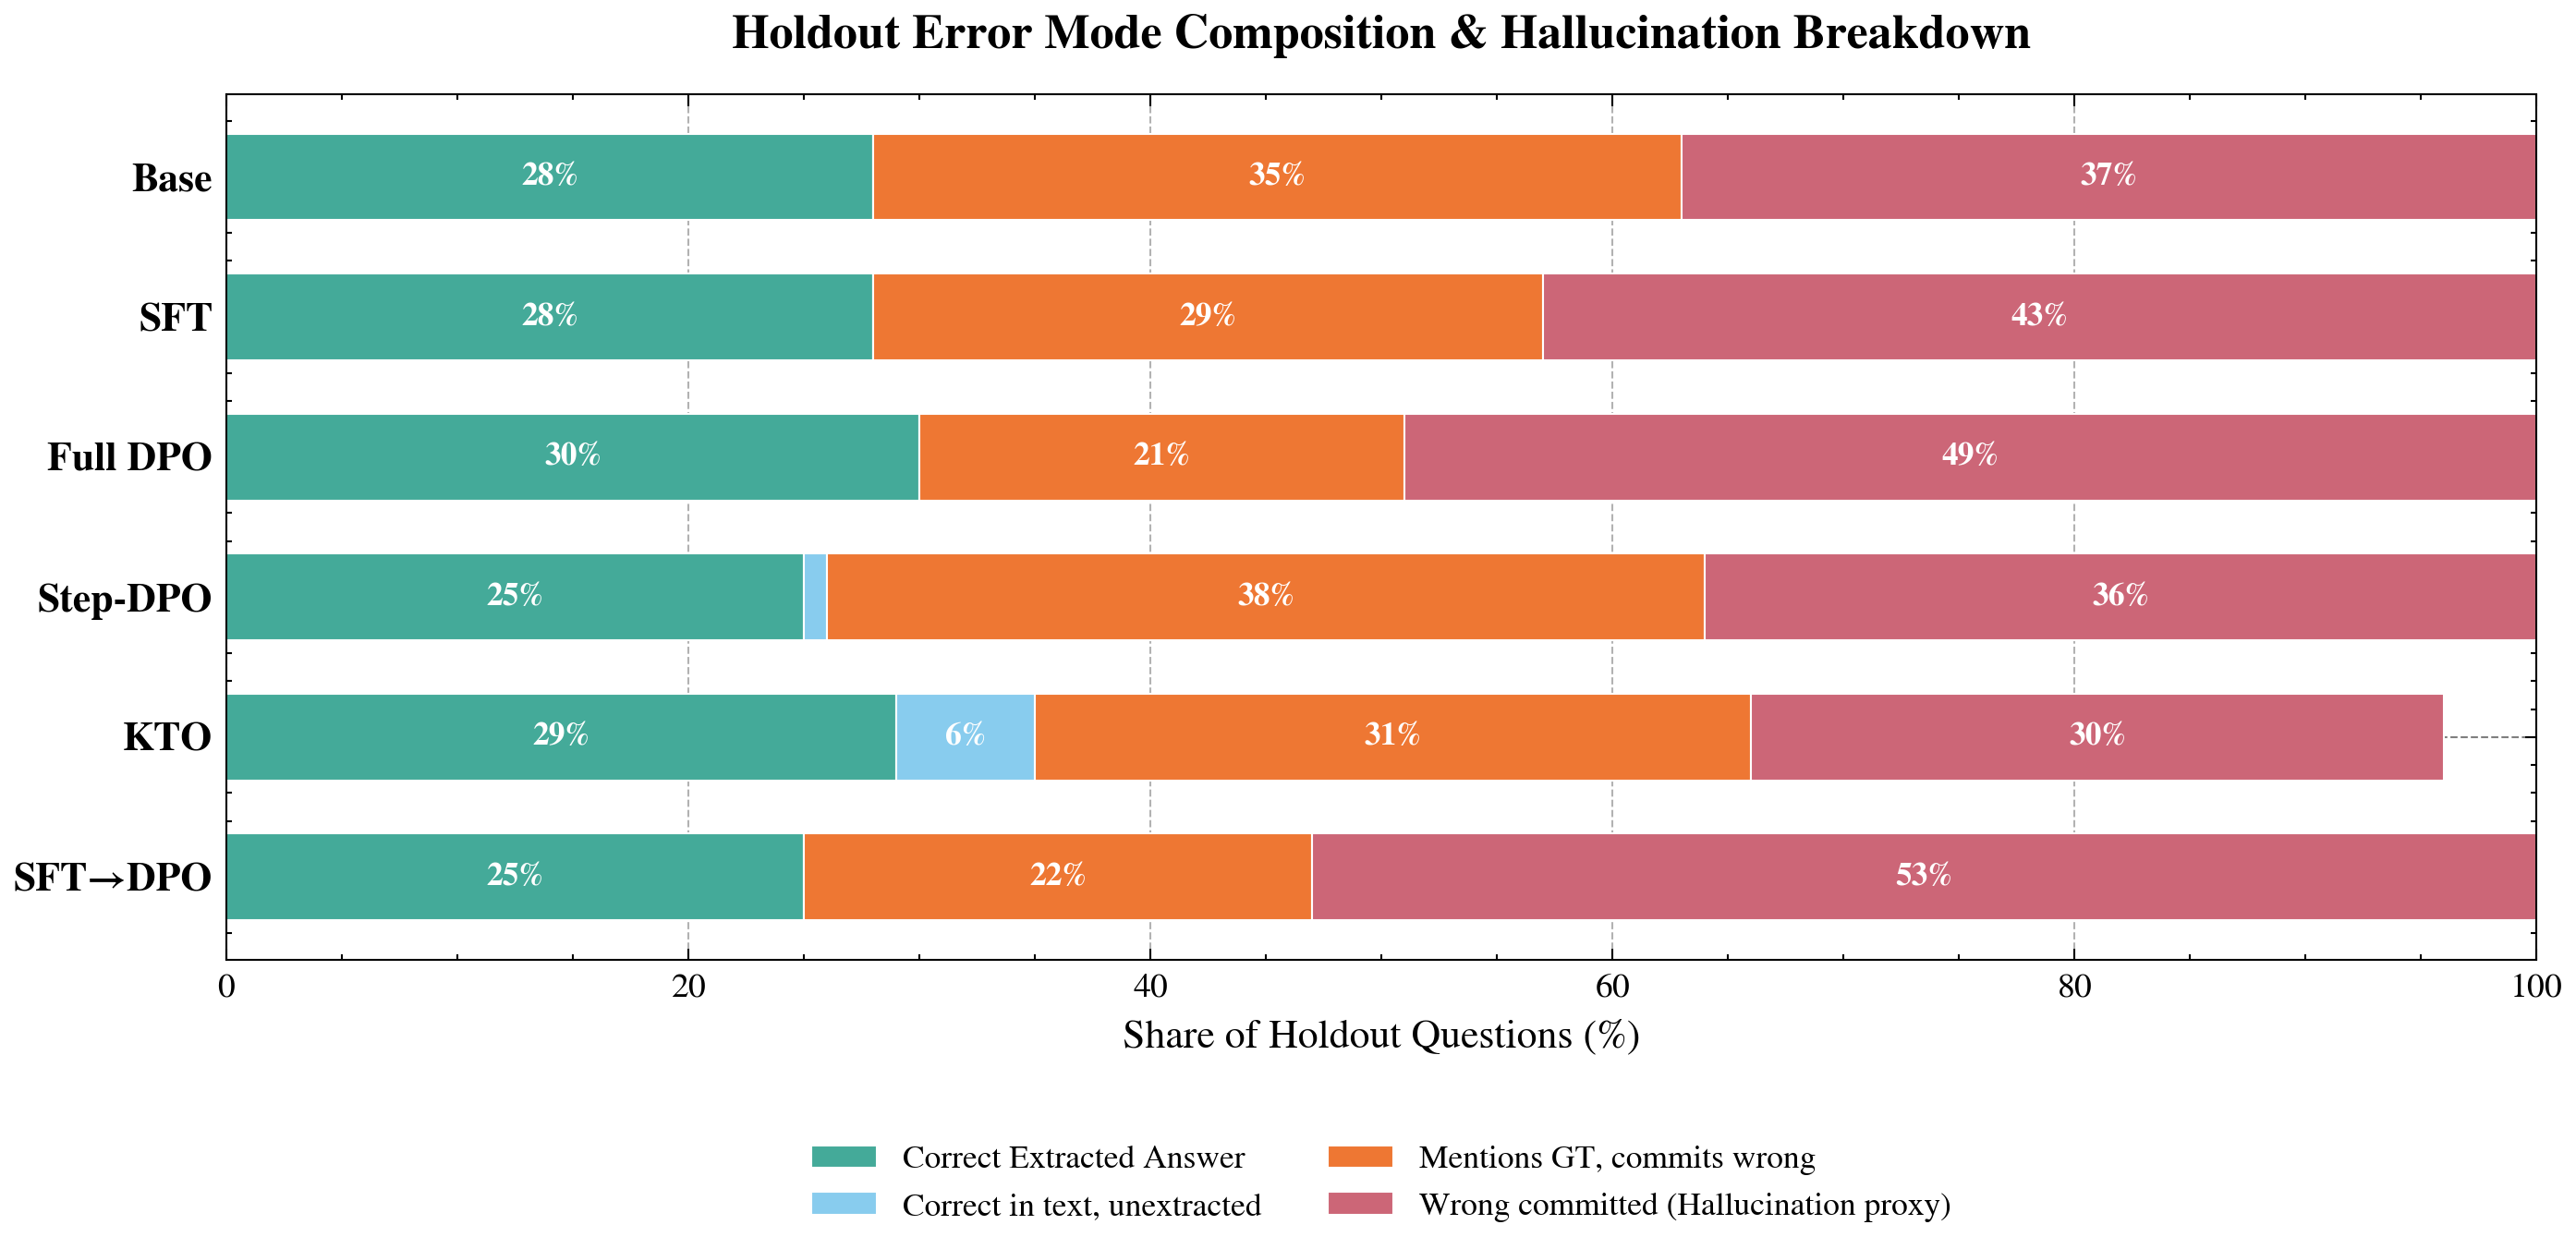
\includegraphics[width=\columnwidth]{../charts/report_selected/results_03_error_mode_hallucination_breakdown.png}
  \caption{\textbf{Holdout Error Mode Breakdown.} Partitioning of test responses into extracted correct, unextracted correct in prose, partial ground-truth mentions, and committed wrong answers (hallucination proxy).}
  \label{fig:error_modes}
\end{figure}

\begin{figure*}[t]
  \centering
  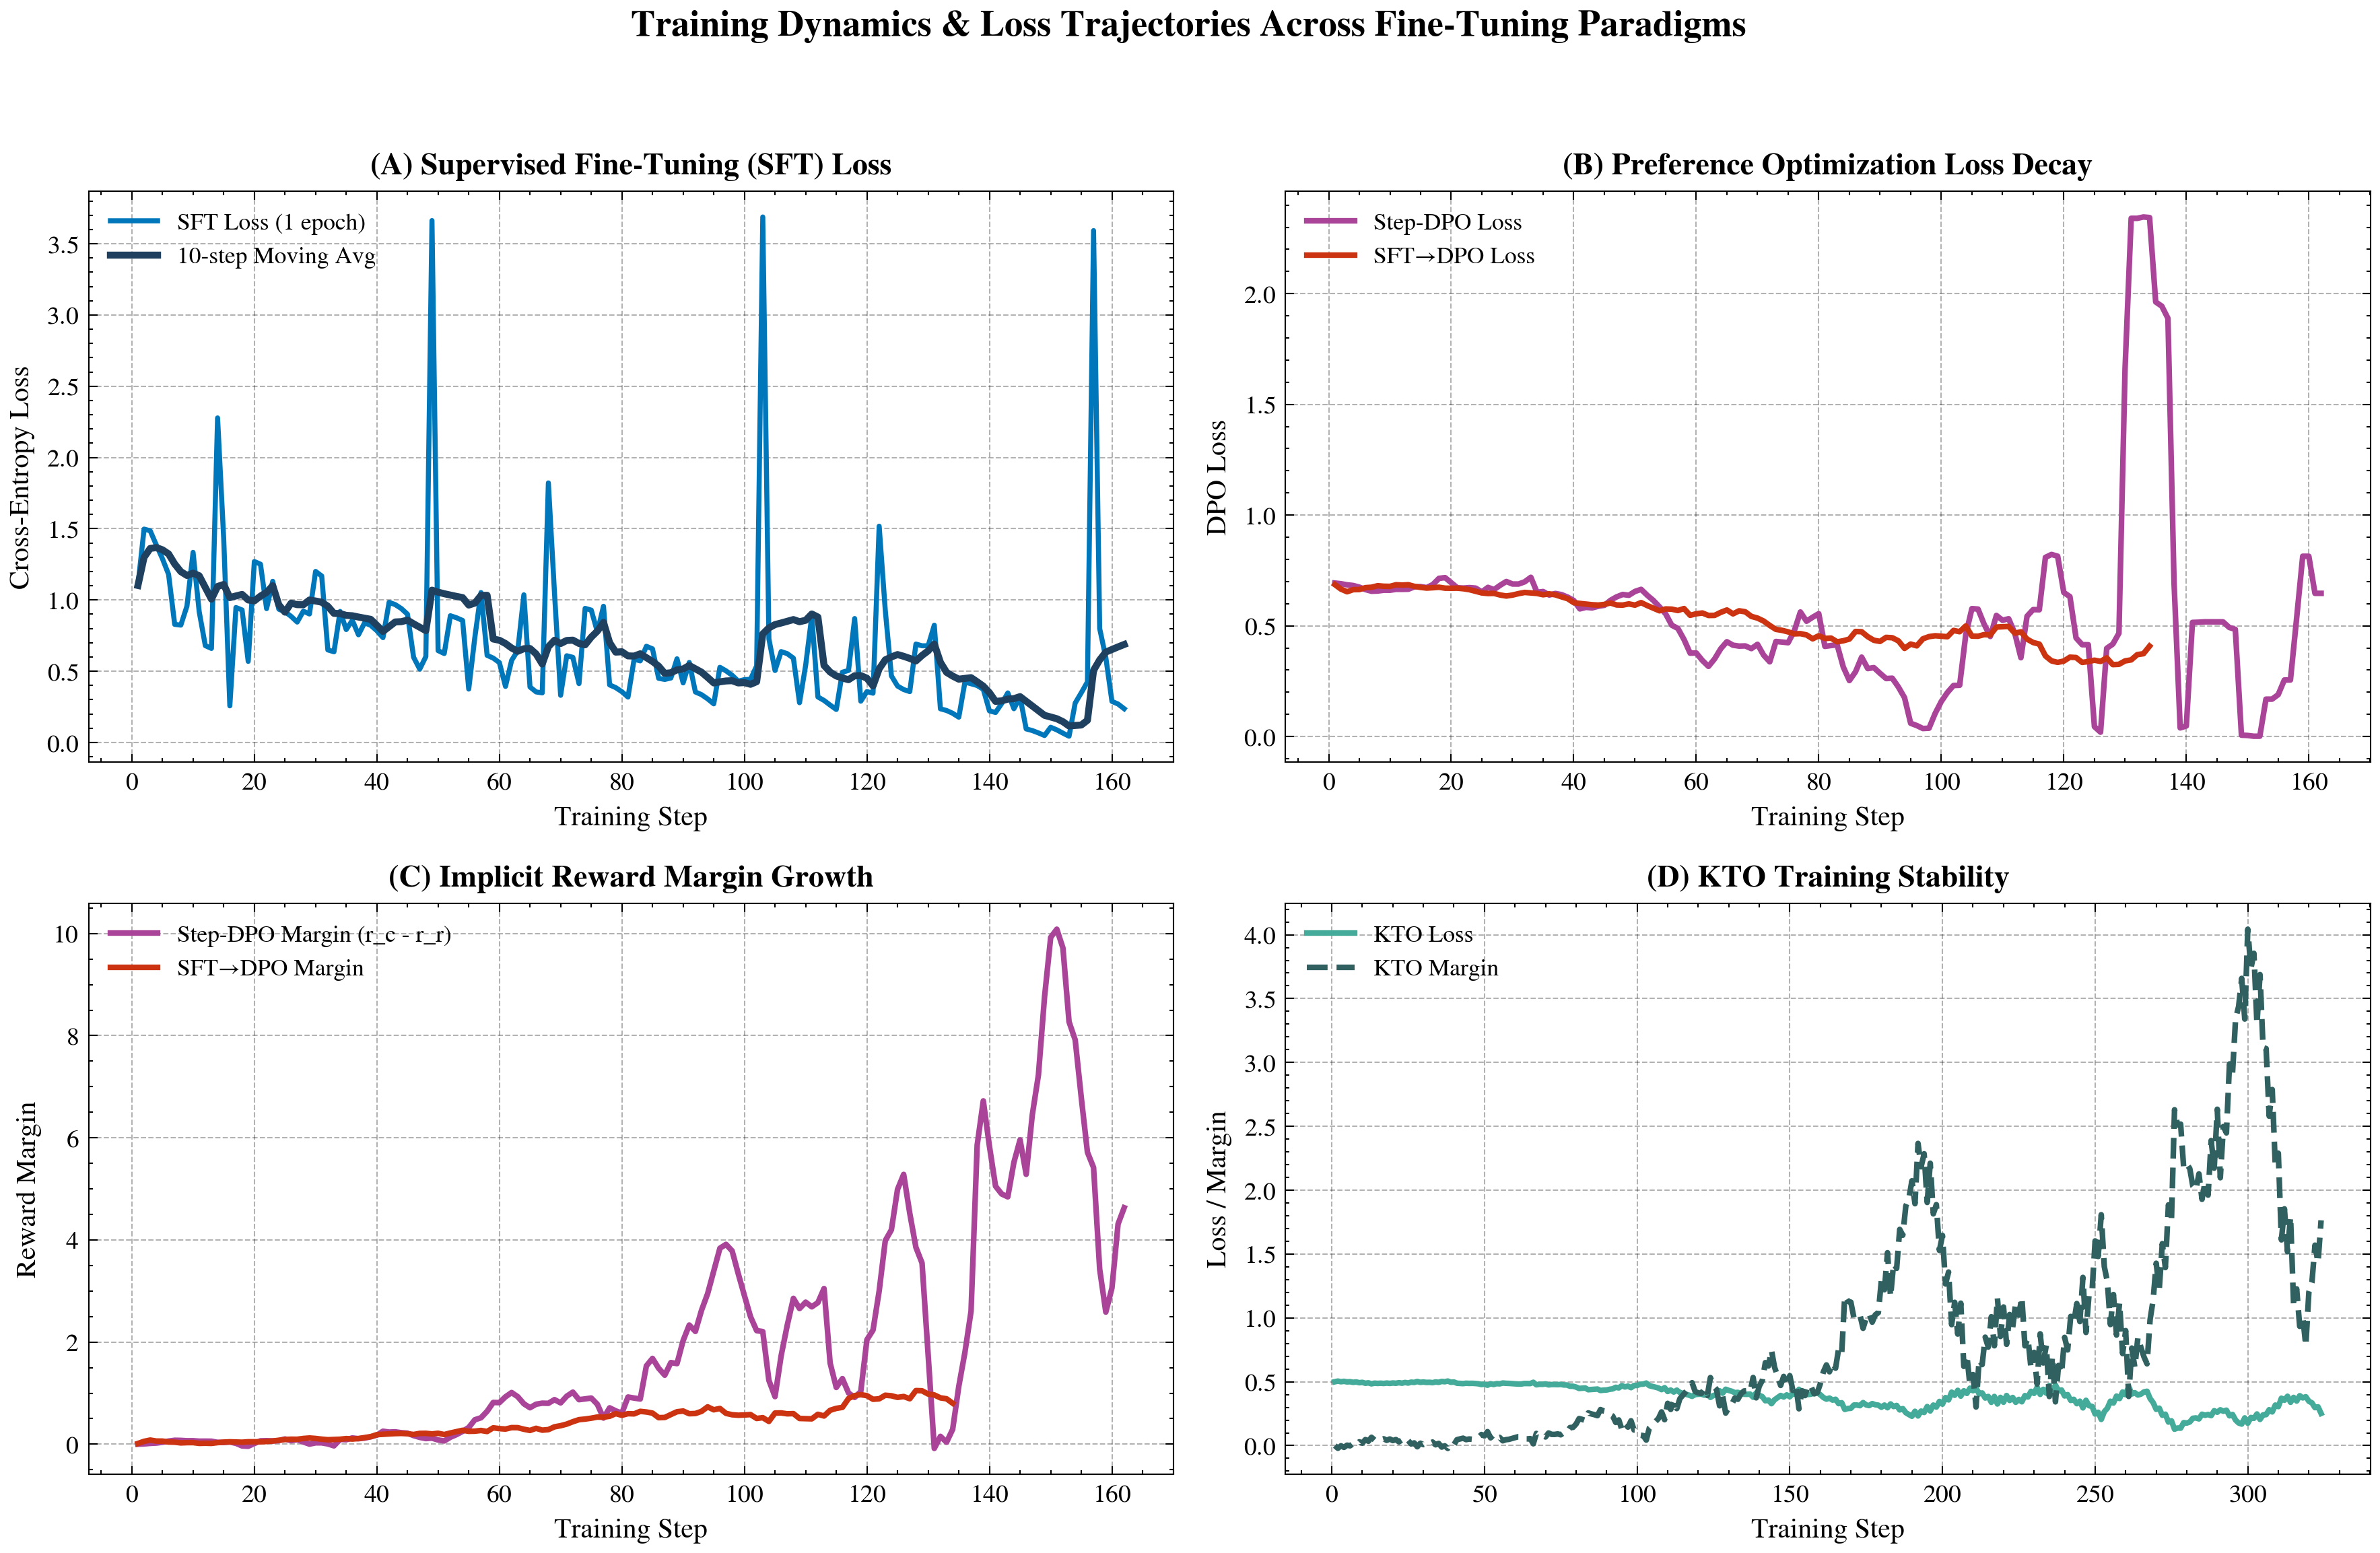
\includegraphics[width=0.90\textwidth]{../charts/report_selected/results_04_training_dynamics_loss_rewards.png}
  \caption{\textbf{Training Dynamics Across Alignment Paradigms.} Top-left: SFT cross-entropy loss decay. Top-right: DPO loss trajectories. Bottom-left: Step-DPO implicit reward margin explosion ($\Delta r \to +10.0$). Bottom-right: KTO margin oscillations under single-T4 GPU constraints.}
  \label{fig:appendix_training_dynamics}
\end{figure*}

\begin{figure}[t]
  \centering
  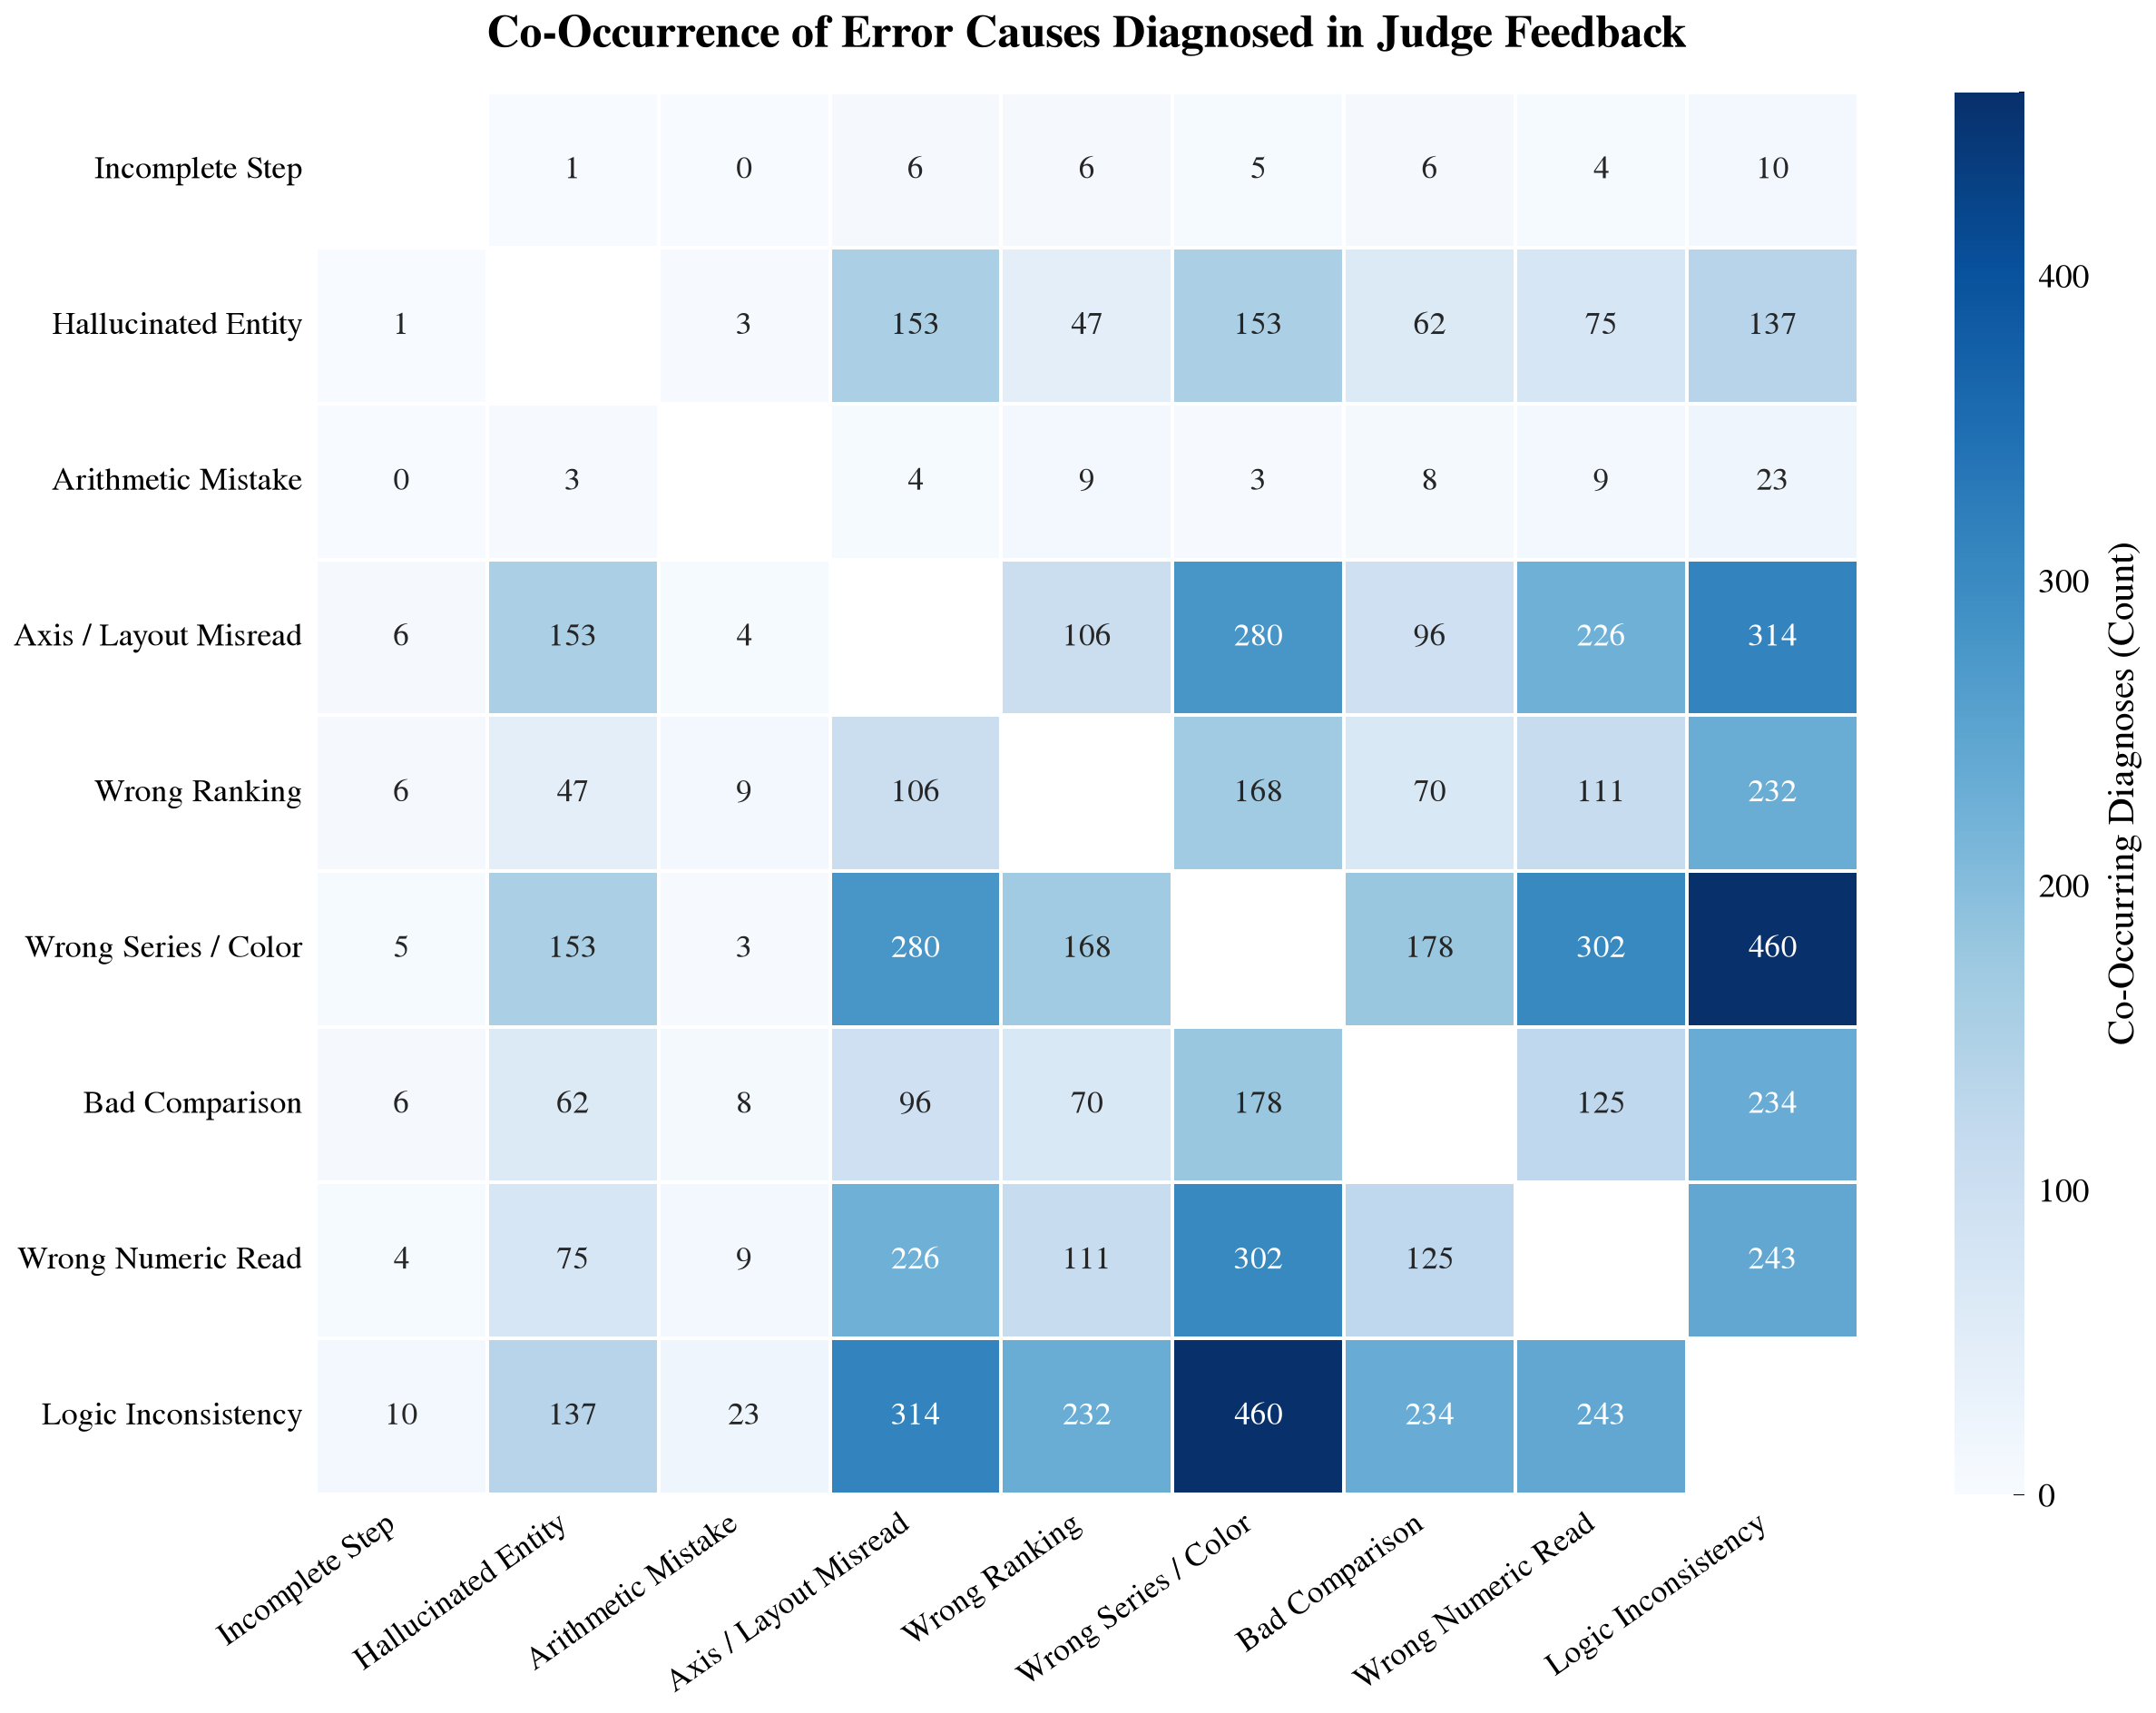
\includegraphics[width=\columnwidth]{../charts/report_selected/judge_07_multilabel_cooccurrence.png}
  \caption{\textbf{Compound Error Co-Occurrence Heatmap.} Off-diagonal counts show strong coupling between perceptual errors and downstream logical failures (460 co-occurrences between logic errors and series confusion).}
  \label{fig:appendix_cooccurrence}
\end{figure}

\begin{figure}[t]
  \centering
  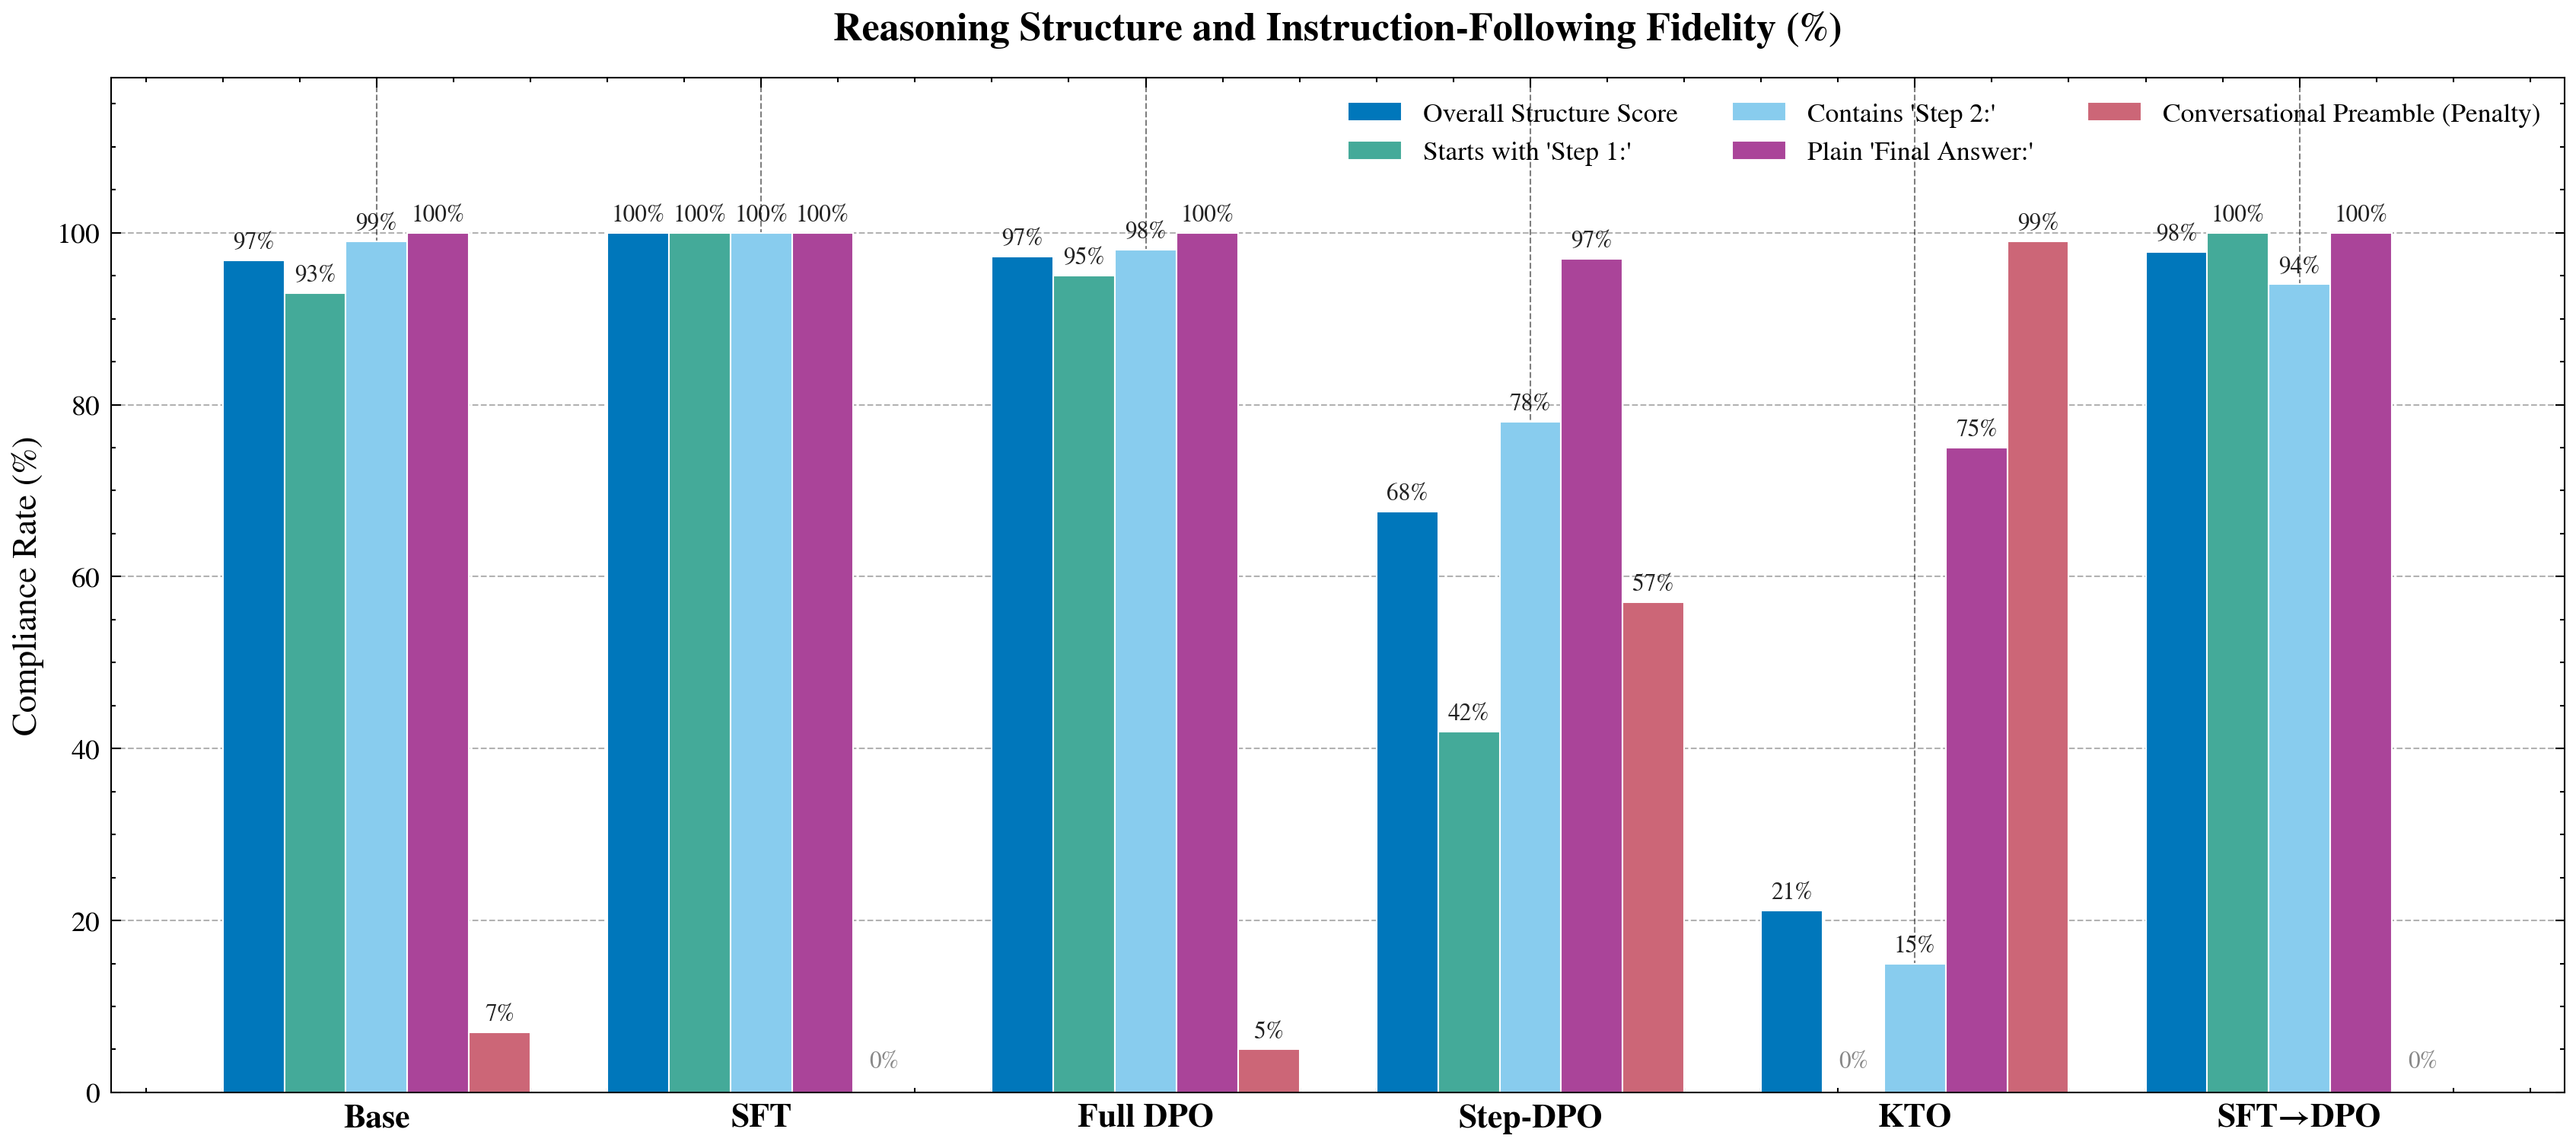
\includegraphics[width=\columnwidth]{../charts/report_selected/results_02_structure_instruction_following.png}
  \caption{\textbf{Structural Instruction Compliance Breakdown.} Evaluates individual prompt constraints. SFT achieves 100\% across all tags, while KTO fails primarily due to conversational preambles and missing answer tags.}
  \label{fig:appendix_structure_breakdown}
\end{figure}

\begin{figure}[t]
  \centering
  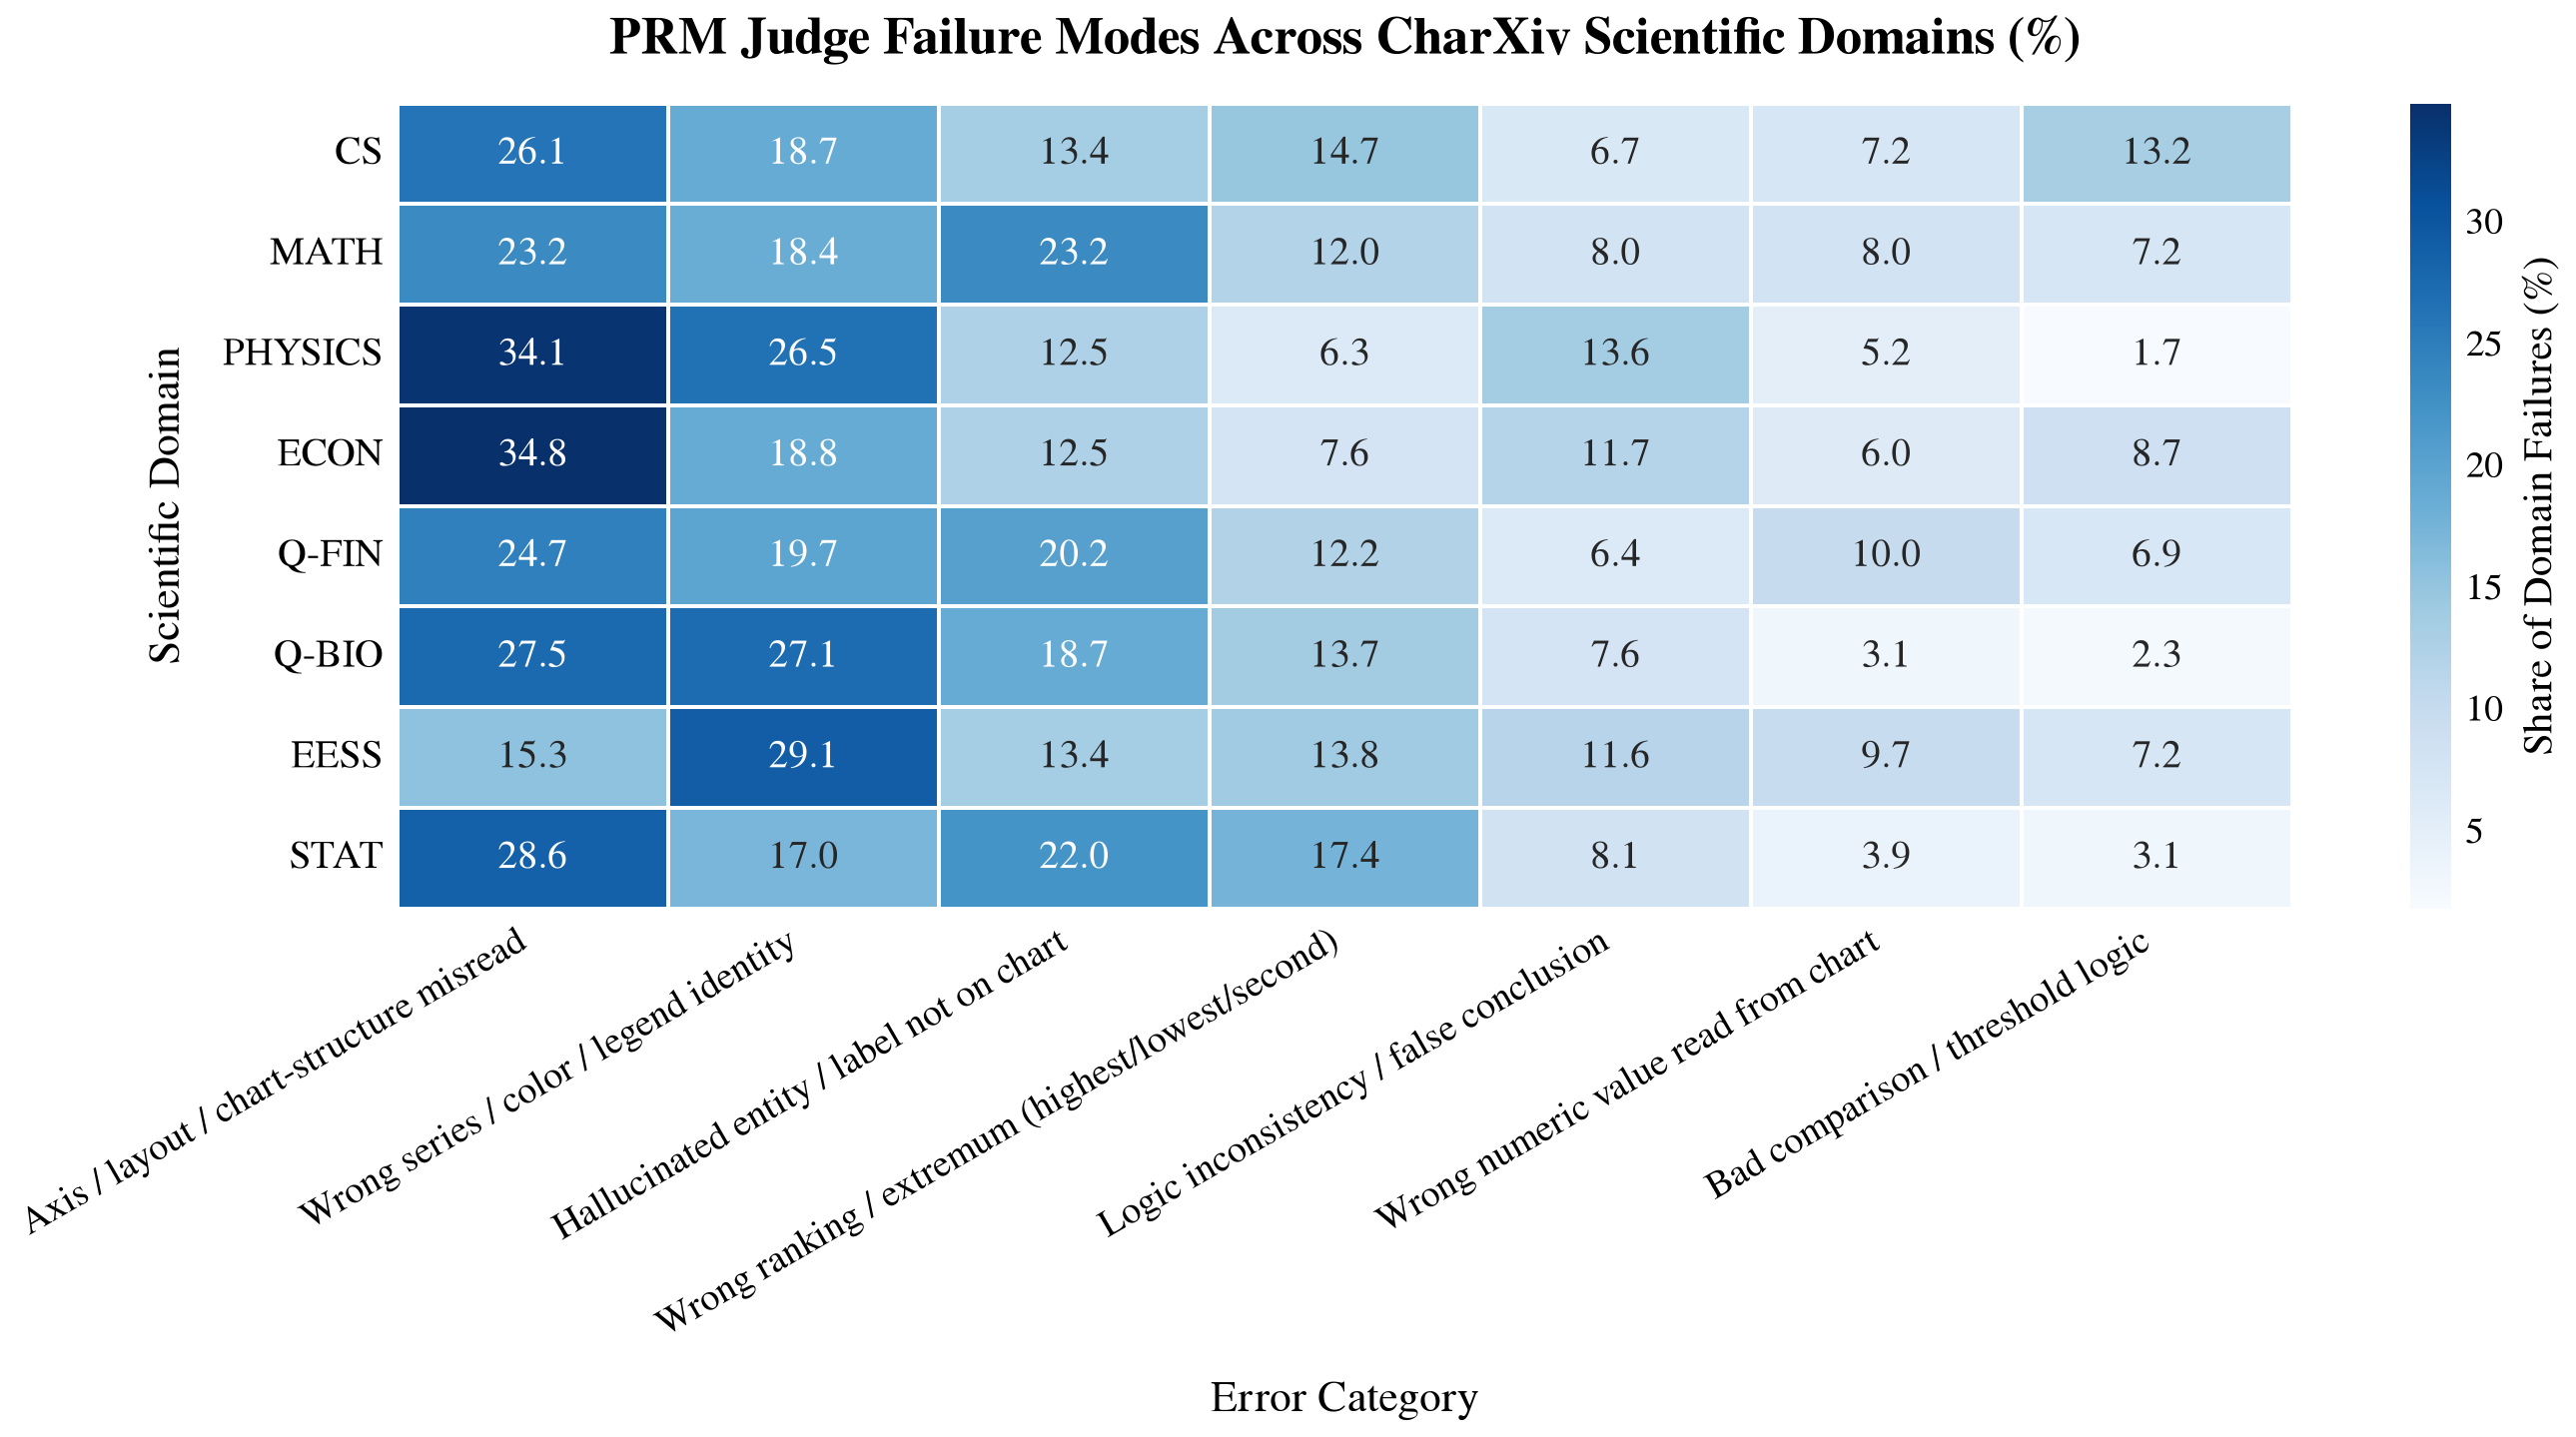
\includegraphics[width=\columnwidth]{../charts/report_selected/judge_05_error_taxonomy_by_domain.png}
  \caption{\textbf{Error Distribution Across CharXiv Domains.} Physics and Economics charts exhibit the highest rate of axis misreads (>34\%), while Mathematics and Computer Science suffer more from entity hallucinations (>22\%).}
  \label{fig:appendix_domain_taxonomy}
\end{figure}

\end{document}
